\documentclass[a4paper,12pt,oneside]{skripsi}

\usepackage[bahasa]{babel}
\usepackage[T1]{fontenc}
\usepackage{setspace}
\usepackage{mathptmx}
\usepackage[latin1]{inputenc}
\setcounter{secnumdepth}{3}
\setcounter{tocdepth}{3}
\usepackage{array}
\usepackage{longtable}
\usepackage{graphicx}
\usepackage{multind}
\usepackage{rotating} %for rotate/sideway text
\usepackage{subfig} %for make floating sub-figure
\usepackage[top=4cm, bottom=3cm, left=4cm, right=3cm]{geometry}

%\makeindex{subject}
\centerchapter
\makeatletter
\newcommand\thefontsize[1]{{#1 The current font size is: \f@size pt\par}}
\makeatother
\parindent 3.0em

\setstretch{1.5}

%===================================================================
% \setlength{\textwidth}{15.0cm}
% \setlength{\evensidemargin}{2.5cm} % outer/right margin
% % \setlength{\topmargin}{0.3cm}    % top margin
% \setlength{\footskip}{2.5cm}       % distance between text and foot
% \setlength{\textheight}{\paperheight}
% \addtolength{\textheight}{-\topmargin}
% \addtolength{\textheight}{-\headheight}
% \addtolength{\textheight}{-\headsep}
% \addtolength{\textheight}{-\footskip}
% \addtolength{\textheight}{-4cm}   % bottom margin
%==============================================================================
\tolerance=1
\emergencystretch=\maxdimen
\hyphenpenalty=10000
\hbadness=10000

\addto\captionsbahasa{
  \renewcommand{\contentsname}{DAFTAR ISI} 
  \renewcommand{\listfigurename}{DAFTAR GAMBAR}
  \renewcommand{\listtablename}{DAFTAR TABEL}
  \renewcommand{\chaptername}{BAB}
  \renewcommand{\chaptername}{BAB}
  \renewcommand{\bibname}{DAFTAR PUSTAKA}
}


\begin{document}

\nocite{*}
%#start bagian administrasi #==================================================
% bagian muka sebelum isi, umumnya halaman administrasi, kalau tidak digunakan
% dapat diberikan tanda % didepannya

%cover
\pagestyle{empty}
\pagenumbering{roman}
\setcounter{page}{1}
\newpage

\addcontentsline{toc}{chapter}{HALAMAN JUDUL}

\begin{center}

\bfseries

{\Large UNIVERSITAS GUNADARMA}\\
{\Large FAKULTAS TEKNOLOGI INDUSTRI}\\

\vspace{1.0cm}

\begin{figure}[h]
  \begin{center}
    
\includegraphics[scale=4.5]{gambar/LogoGunadarma.jpg}
  \end{center}
\end{figure}

{\large ESTIMASI POSE TIGA DIMENSI DARI GAMBAR MONOKULER MENGGUNAKAN DEEP NEURAL NETWORK}

\vspace{1.5cm}

\begin{tabular}{|c|}
  \hline
  Disusun oleh: \\
  \begin{tabular}{ll}
  Nama& : Denilson \\[-5pt]
  NPM& : 51416815 \\[-5pt]
  Jurusan& : Teknik Informatika \\[-5pt]
  Pembimbing& : Dr. Dharmayanti, ST., MMSI.\\
  \end{tabular}\\
  \hline
\end{tabular}

\end{center}

\vspace{1.5cm}

\begin{center}
\bfseries
Diajukan Guna Melengkapi Sebagian Syarat \\
Dalam Mencapai Gelar Sarjana Strata Satu (S1)\\

Depok\\
2020 %DIGANTI TAHUN PENULISAN SKRIPSI
\end{center}



%halaman lembar pengesahan, abstraksi, kata pengantar
\pagestyle{plain}
\pagenumbering{roman}
\setcounter{page}{2} %nilai halaman utk awal dari abstrak s/d ucapan terimakasih dlm romawi


\newpage
\addcontentsline{toc}{chapter}{LEMBAR ORIGINALITAS DAN PUBLIKASI}
\begin{center}
    {\large \bf \centering LEMBAR ORIGINALITAS DAN PUBLIKASI}
    \vspace{0.75cm}
\end{center}

\noindent Saya yang bertanda tangan di bawah ini,
\vspace{0.5cm}

\begin{flushleft}
    \begin{tabular}{ll}
        Nama                   & : Denilson                                         \\
        NPM                    & : 51416815                                         \\
        Judul Penulisan Ilmiah & : Estimasi Pose Tiga Dimensi dari Gambar Monokuler \\
                               & \hspace{5pt} Menggunakan Deep Neural Network       \\
        Tanggal Sidang         & : tanggal                                          \\
        Tanggal Lulus          & : tanggal                                          \\
    \end{tabular}
\end{flushleft}

\vspace{0.5cm}

\noindent menyatakan bahwa tulisan ini adalah merupakan hasil karya saya sendiri dan dapat
dipublikasikan sepenuhnya oleh Universitas Gunadarma. Segala kutipan dalam bentuk apa pun telah
mengikuti kaidah, etika yang berlaku. Mengenai isi dan tulisan adalah merupakan tanggung jawab
penulis, bukan Universitas Gunadarma.

\vspace{0.5cm}

\noindent Demikian pernyataan ini dibuat dengan sebenarnya dan dengan penuh kesadaran.

\begin{flushright}
    Jakarta, April 2020

    \vspace{2cm}

    Denilson
\end{flushright}

\newpage
\addcontentsline{toc}{chapter}{LEMBAR PENGESAHAN}
\begin{center}
{\large \bf \centering LEMBAR PENGESAHAN}

\vspace{0.75cm}

{\bf Komisi Pembimbing}

\vspace{0.5cm}

\begin{tabular}{|c|c|c|}
\hline
No & Nama & Kedudukan\\
\hline

 1& Dr. Dharmayanti, ST., MMSI.& Ketua \\
 \hline

 2& DIGANTI NAMA PENGUJI 2& DIGANTI JABATAN PENGUJI 2\\
 \hline
 3& DIGANTI NAMA PENGUJI 3& DIGANTI JABATAN PENGUJI 3\\
 \hline
\end{tabular}

\vspace{0.1cm}
\begin{flushright}
{Tanggal Sidang : tgl bln thn}
\end{flushright}

\vspace{0.5cm}

{\bf Panitia Ujian}

\vspace{0.5cm}

\begin{tabular}{|c|c|c|}
\hline
No & Nama & Kedudukan\\
\hline

 1& DIGANTI NAMA PENGUJI 1& DIGANTI JABATAN PENGUJI 1\\
 \hline

 2& DIGANTI NAMA PENGUJI 2& DIGANTI JABATAN PENGUJI 2\\
 \hline
 3& DIGANTI NAMA PENGUJI 3& DIGANTI JABATAN PENGUJI 3\\
 \hline
 4& DIGANTI NAMA PENGUJI 4& DIGANTI JABATAN PENGUJI 4\\
 \hline
 5& DIGANTI NAMA PENGUJI 5& DIGANTI JABATAN PENGUJI 5\\
 \hline
\end{tabular}

\vspace{0.1cm}
\begin{flushright}
{Tanggal Lulus : tgl bln thn}
\end{flushright}

{\bf MENGETAHUI}

\vspace{0.5cm}

{Pembimbing~ \hspace{5.0cm} ~Bagian Sidang Sarjana}%

\vspace{1.5cm}

{(Dr. Dharmayanti, ST., MMSI.)~ \hfill ~(NAMA BAGIAN SARJANA)}%


\end{center}
% menggabungkan file lembar pengesahan

\newpage %Abstract
\addcontentsline{toc}{chapter}{ABSTRAKSI}
\begin{center}
\begin{large}\textbf{ABSTRAKSI}\end{large}
\end{center}

\vspace{5mm} 

\noindent \textbf{Denilson}, 51416815 \\
\textbf{ESTIMASI POSE TIGA DIMENSI DARI GAMBAR MONOKULER MENGGUNAKAN DEEP NEURAL NETWORK}\\
\textbf{Tugas Akhir}. Jurusan Teknik Informatika, Fakultas Teknologi Industri, \\
Universitas Gunadarma, 2020\\
Kata Kunci : dibuat urut abjad sekitar 3-5 kata kunci\\
\noindent (jml hlm romawi + jml hlm arab + Lampiran)\\

\setstretch{1.0}
Abstraksi bla bla bla bla, ini sangat tidak hebat hahahahhaha.
Abstraksi bla bla bla bla, ini sangat tidak hebat hahahahhaha.
Abstraksi bla bla bla bla, ini sangat tidak hebat hahahahhaha.
Abstraksi bla bla bla bla, ini sangat tidak hebat hahahahhaha.
Abstraksi bla bla bla bla, ini sangat tidak hebat hahahahhaha.
Abstraksi bla bla bla bla, ini sangat tidak hebat hahahahhaha.
Abstraksi bla bla bla bla, ini sangat tidak hebat hahahahhaha.
Abstraksi bla bla bla bla, ini sangat tidak hebat hahahahhaha.
Abstraksi bla bla bla bla, ini sangat tidak hebat hahahahhaha.
Abstraksi bla bla bla bla, ini sangat tidak hebat hahahahhaha.\\

\setstretch{1.5}
\noindent Daftar Pustaka (thn terlama-thn terbaru)
% menggabungkan file abstraksi

%menggabungkan file CV atau riwayat hidup ringkas
%\newpage %CV
\addcontentsline{toc}{section}{Riwayat Hidup}

\begin{center}
\begin{large}\textbf{Riwayat Hidup}\\\end{large}
\end{center}
\vspace{5mm}

\begin{tabular}{ll}
Nama&
DIGANTI NAMA PENULIS\tabularnewline
Tanggal Lahir&
DIGANTI TEMPAT, TANGGAL LAHIR\tabularnewline
Pendidikan Formil&
DIGANTI PENDIDIKAN FORMIL TERAKHIR\tabularnewline
Pendidikan Non-Formil&
DIISI JIKA ADA DENGAN PENDIDIKAN NON-FORMIL TERAKHIR\tabularnewline
\end{tabular}
\newpage %Acknowledgment
\addcontentsline{toc}{chapter}{KATA PENGANTAR}
\begin{center}
  \begin{large}\textbf{KATA PENGANTAR}\\\end{large}
\end{center}
\vspace{5mm}


Segala puji dan syukur penulis ucapkan ke hadirat Tuhan Yang Maha Esa yang telah memberikan berkat,
anugerah dan karunia yang melimpah, sehingga penulis dapat menyelesaikan tugas akhir ini pada waktu
yang telah ditentukan.

Tugas akhir ini disusun guna melengkapi sebagian syarat untuk memperoleh gelar Sarjana Teknik
Informatika Universitas Gunadarma. Adapun judul tugas akhir ini adalah "Estimasi Pose Tiga Dimensi
Dari Gambar Monokuler Menggunakan Deep Neural Network".

Walaupun banyak kesulitan yang penulis harus hadapi ketika menyusun tugas akhir ini, namun berkat
bantuan dan dorongan dari berbagai pihak, akhirnya tugas akhir ini dapat diselesaikan dengan baik.
Untuk itu penulis tidak lupa mengucapkan terima kasih kepada:

\begin{enumerate}
  \item Prof. Dr. E. S. Margianti, SE., MM., selaku Rektor Universitas Gunadarma.
  \item Prof. Dr. -Ing. Adang Suhendra, SSi., S.Kom., M.Sc., selaku Dekan Fakultas Teknologi Industri Universitas Gunadarma.
  \item Dr. Lintang Yuniar Banowosari, S.Kom., M.Sc., selaku Ketua Jurusan Fakultas Teknik Informatika Universitas Gunadarma.
  \item Dr, Edi Sukirman, SSi., MM., selaku Kepala Bagian Sidang Ujian Universitas Gunadarma.
  \item Dr. Dharmayanti, ST., MMSI., sebagai dosen pembimbing penulis yang ditengah-tengah kesibukannya
        telah membimbing penulis sehingga penulisan ini dapat diselesaikan.
  \item Keluarga yang selalu mendukung dan terus memberikan motivasi.
  \item Semua pihak yang terlibat dalam membantu penyelesaian Tugas Akhir ini.

\end{enumerate}

Sebagai manusia biasa yang tak luput dari kesalahan, maka penulis meminta maaf atas segala
kekurangan dan keterbatasan dalam penyusunan tugas akhir ini. Penulis sadari bahwa penulisan ini
masih jauh dari sempurna, disebabkan karena berbagai keterbatasan yang penulis miliki. Untuk itu
penulis mengharapkan kritik dan saran yang bersifat membangun untuk menjadi perbaikan di masa yang
akan datang.

Akhir kata, penulis berharap penulisan ini dapat bermanfaat bagi semua pihak dan bagi penulis
pribadi khususnya, serta dapat digunakan sebagaimana mestinya.


\vspace{0.5 cm}
\begin{flushright}
  Jakarta, April 2020

  \vspace{2 cm}
  Denilson
\end{flushright}% mengabungkan file kata pengantar

%# akhir bagian administrasi # ==========================================

% #mulai membuat daftar isi, daftar gambar dan  daftar tabel # ==========
%\setcounter{page}{8} %set nilai halaman sesuai urutannya

% membuat daftar isi
\tableofcontents{}
\addcontentsline{toc}{chapter}{DAFTAR ISI}

%% membuat daftar tabel
\listoftables
\addcontentsline{toc}{chapter}{DAFTAR TABEL}

%membuat daftar gambar
\listoffigures
\addcontentsline{toc}{chapter}{DAFTAR GAMBAR}%masih masalah

\newpage %lampiran
\addcontentsline{toc}{chapter}{DAFTAR LAMPIRAN}
\begin{center}
    \begin{large}\textbf{DAFTAR LAMPIRAN}\\\end{large}
\end{center}
\vspace{5mm}
\noindent Lampiran 1: Kelas Dataset
. . . . . . . . . . . . . . . . . . . . . . . . . . . . . . . . . . . . . . L1

\noindent Lampiran 2: Kelas ResLinear
. . . . . . . . . . . . . . . . . . . . . . . . . . . . . . . . . . . . L1

\noindent Lampiran 3: Arsitektur Model
. . . . . . . . . . . . . . . . . . . . . . . . . . . . . . . . . . . .L1

\noindent Lampiran 4: Options
. . . . . . . . . . . . . . . . . . . . . . . . . . . . . . . . . . . . . . . . . . L2

\noindent Lampiran 5: Pemuatan Data
. . . . . . . . . . . . . . . . . . . . . . . . . . . . . . . . . . . . . L2

\noindent Lampiran 6: Instansiasi Dataset dan DataLoader
. . . . . . . . . . . . . . . . . . . . . . .L2

\noindent Lampiran 7: Algoritma Pelatihan
. . . . . . . . . . . . . . . . . . . . . . . . . . . . . . . . . L2

\noindent Lampiran 8: Algoritma Validasi
. . . . . . . . . . . . . . . . . . . . . . . . . . . . . . . . . . L2

\noindent Lampiran 9: Instansiasi Model
. . . . . . . . . . . . . . . . . . . . . . . . . . . . . . . . . . . L2

\noindent Lampiran 10: Visualisasi Titik Kunci
. . . . . . . . . . . . . . . . . . . . . . . . . . . . . . .L3

\noindent Lampiran 11: Visualisasi Inferensi
. . . . . . . . . . . . . . . . . . . . . . . . . . . . . . . . L3

\noindent Lampiran 12: Plot Grafik
. . . . . . . . . . . . . . . . . . . . . . . . . . . . . . . . . . . . . . . L3

% #akhir membuat daftar isi, daftar gambar dan  daftar tabel # ==========

% # mulai bagian isi # ==================================================

\newpage
\pagestyle{plain}
\pagenumbering{arabic} % jenis huruf arabic
\setcounter{page}{1} %mulai dari halaman 1



\chapter{PENDAHULUAN}
\label{cha:1-Pendahuluan}

\section{Latar Belakang Masalah}
\label{sec:1-LatarBelakangMasalah}

Pemanfaatan teknologi yang terkomputerisasi oleh manusia selalu meninggalkan jejak yang
tersimpan dalam bentuk data digital. Rekam jejak ini merupakan bukti perilaku dan karakteristik
manusia  sehingga dijadikan acuan pengembangan teknologi dan ilmu pengetahuan pada masa mendatang.
Data digital yang umumnya dimanfaatkan oleh manusia meliputi teks, citra audio, citra visual, dan
citra audio visual yang disimpan ke dalam suatu media penyimpanan. Jumlah data yang tersedia
tergolong banyak dan akan semakin bertambah seiring dengan gaya hidup manusia yang semakin
bergantung pada teknologi digital.

Jejak digital bersifat laten yang berarti data digital memiliki makna khusus dan hanya dapat diolah
dengan prosedur khusus. Citra visual terbentuk dari penangkapan pantulan gelombang elektromagnetik
benda yang berada depan kamera dan kemudian disimpan dalam bentuk digital. Hasil akhir citra visual
yang tercipta hanya memiliki informasi numerik mengenai warna, sedangkan
informasi posisi benda saat penangkapan sudah hilang. Otak manusia dapat mengartikan kondisi suatu
benda dalam suatu gambar tanpa diketahui cara kerjanya secara pasti. Hal yang sama dapat
dilakukan komputer dengan membuat fungsi pemetaan dari suatu gambar terhadap suatu kondisi dengan
memanfaatkan data gambar dalam jumlah besar sebagai acuan.

Permodelan pemelajaran dalam atau \textit{deep learning} dapat memetakan suatu domain ke
domain lainnya secara mandiri menggunakan pemelajaran jaringan saraf tiruan dalam atau
\textit{deep neural network}. Pemelajaran dalam menggunakan jaringan
saraf tiruan dapat digunakan untuk memajukan teknologi khususnya di bidang visi komputer
seperti melakukan estimasi pose tiga dimensi tubuh manusia yang terdapat dalam suatu gambar.

\section{Rumusan Masalah}
\label{sec:1-RumusanMasalah}
Permasalahan yang ingin diselesaikan adalah mengestimasi pose tubuh manusia yang
telah hilang dengan membuat sebuah pemetaan dari gambar yang ditangkap kamera monokuler ke
koordinat setiap titik kunci dari pose menggunakan model \textit{deep neural network}.
Model yang telah terlatik mampu melakukan proses
pemetaan terhadap gambar baru sehingga dapat dijadikan sebagai acuan aplikasi pembaca pose tubuh
manusia dari gambar monokuler.

\section{Batasan Masalah}
\label{sec:1-BatasMasalah}

Penelitian ini menganggap setiap pose dua dimensi maupun pose tiga dimensi berada dalam koordinat
lokal. Setiap pose ditransformasi ke dalam sistem koordinat kamera dengan titik kunci pinggang
sebagai titik koordinat tengah. Hal ini dilakukan karena pemetaan hanya menggunakan gambar dua dimensi
tanpa informasi kedalaman titik kunci sehingga dapat mengesampingkan masalah kedalaman yang ambigu.

\section{Tujuan Penelitian}
\label{sec:1-TujuanPenelitian}

Tujuan dari penelitian ini adalah untuk membuat sebuah aplikasi yang dapat mengestimasi titik kunci dari
sebuah citra visual datar dan melakukan transformasi ke pose lokal dua dimensi sehingga dapat
dipetakan oleh jaringan saraf tiruan yang dimodelkan ke bentuk pose lokal tiga dimensi. Pose hasil
juga divisualisasikan secara interaktif sehingga dapat digunakan untuk kepentingan yang sesuai.

\section{Metode Penelitian}
\label{sec:1-MetodePenelitian}

Penelitian dibagi menjadi tiga tahap besar terurut yang terdiri dari \textit{data preprocessing},
pelatihan model jaringan saraf tiruan, dan visualisasi. Tahap pertama dan tahap ketiga tidak
melibatkan pemelajaran mesin. Permasalahan utama dari penelitian ini berada pada tahap kedua tentang
pelatihan jaringan saraf tiruan untuk melakukan pemetaan pose dua dimensi ke pose tiga dimensi.

\textit{Dataset} yang digunakan dalam penelitian ini adalah \textit{Human3.6M} yang berisi 3,6 juta
pose unik yang dilakukan oleh sebelas aktor profesional dan direkam menggunakan empat sudut kamera
yang berbeda beserta dengan koordinat setiap titik kunci dari hasil penangkapan alat
\textit{motion capture}~\cite{h36m_pami}.

Pose dua dimensi dan tiga dimensi merupakan variabel yang relevan untuk masalah. Pada tahap
\textit{data preprocessing} akan dilakukan ekstraksi variabel ini menjadi bentuk numerik sehingga
mudah untuk digunakan saat melakukan pelatihan jaringan saraf tiruan. Tahap selanjutnya akan
dilakukan pembuatan, permodelan, pelatihan, dan evaluasi jaringan saraf tiruan dalam untuk
pemetaan titik kunci yang kemudian dilanjutkan dengan percobaan model dengan video. Tahap terakhir
menampilkan visualisasi gambar, pose dua dimensi, dan pose tiga dimensi.

Perangkat keras yang digunakan dalam penelitian ini adalah satu unit laptop dengan spesifikasi:
\begin{itemize}
    \item CPU Intel Core I7 7700HQ
    \item Memori 24 GB DDR4
    \item GPU NVIDIA GTX 1060 6GB
    \item SSD NVME SAMSUNG 120 GB
    \item HDD SATA 1 TB
\end{itemize}

Perangkat lunak yang digunakan dalam penelitian ini adalah satu unit laptop dengan spesifikasi:
\begin{itemize}
    \item Python 3.7
    \item Jupyter Lab
    \item Git
    \item GitHub
    \item LaTeX
\end{itemize}

\section{Sistematika Penulisan}
\label{sec:1-SistematikaPenulisan}

Adapun sistematika penulisan yang digunakan dalam penulisan ini adalah sebagai berikut:

PENDAHULUAN, mengemukakan latar belakang masalah, rumusan masalah, batasan masalah, tujuan
penelitian, metode penelitian, dan sistematika penulisan.

TINJAUAN PUSTAKA, menjelaskan kumpulan teori yang digunakan dalam mendukung proses penyelesaian
program.

PENDEKATAN, mengemukakan langkah-langkah yang dicapai untuk membuat program.

HASIL DAN ANALISIS, mendalami hasil yang tercapai dengan analisis secara mendalam.

PENUTUP, mengulas lebih lanjut mengenai kesimpulan yang dapat ditarik dari hasil disertai dengan
saran yang dapat menyempurnakan penelitian selanjutnya. %Bab 1.Pendahuluan



\chapter{TINJAUAN PUSTAKA}
\label{cha:2-TinjauanPustaka}

\section{Teorema Penaksiran Universal}
\label{sec:2-TeoremaPenaksiranUniversal}

Teorema penaksiran universal atau \textit{universal approximation theorem} menyatakan bahwa sebuah
model jaringan \textit{feed-forward} dapat membentuk fungsi apapun secara subjektif. Sebuah model
jaringan saraf tiruan dibentuk dari serangkaian lapisan yang didalamnya terdapat deretan sel saraf
atau \textit{neuron} dengan kuantitas tertentu. Semakin panjang rangkaian lapisan yang tersedia,
maka semakin banyak saraf yang tersedia sehingga dapat memetakan fungsi yang sulit.
Model jaringan yang memiliki banyak saraf dapat mempelajari pola-pola yang ada dari satu
domain ke domain lainnya~\cite{2016arXiv160100013G}.

Teorema penaksiran universal memiliki dua sifat yang dikategorikan berdasarkan pemanfaatannya dalam
melakukan pemelajaran mesin. Sifat pertama adalah suatu model jaringan saraf tiruan dapat
memperkirakan suatu fungsi dengan batasan-batasan tertentu sesuai dengan fungsi keluaran pada setiap
lapisan yang terdapat dalam model khususnya lapisan yang terdapat pada bagian akhir.
Sifat kedua adalah sebuah fungsi kontinu dengan jumlah variabel sembarang dapat
ditiru sifatnya oleh sebuah jaringan saraf tiruan dengan jumlah parameter yang sembarang~\cite{2019arXiv191003344K}.

\begin{figure}[htbp]
    \begin{center}
        \fbox{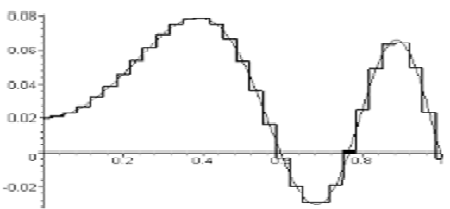
\includegraphics[scale=1.0]{bab2/gambar/uat.png}}
    \end{center}
    \vspace{-20pt}
    \captionsetup{labelfont=bf, textfont=bf}
    \caption{Teorema Penaksiran Universal}
    \vspace{-10pt}
    \captionsetup{labelfont=md, textfont=md}
    \caption*{Sumber: https://encrypted-tbn0.gstatic.com/images?q=tbn}
    % \caption*{Sumber: Zhang (2019)}
    \label{fig:uat}
\end{figure}

\section{Jaringan Saraf}
\label{sec:2-JaringanSaraf}

Otak manusia terdiri dari kumpulan sel saraf yang saling terkoneksi satu sama lain. Sebuah sel saraf
adalah sel yang dapat memproses dan mengantarkan informasi apabila dirangsang dengan tegangan
elektrokimia. Sel-sel saraf tidak membelah dirinya dan tidak digantikan apabila ada yang
rusak. Jumlah sel saraf yang terdapat dalam otak manusia diperkirakan sebanyak satu miliar. Setiap
sel saraf diperkirakan berkoneksi dengan sepuluh ribu sel saraf lainnya melalui sinapsis yang
berarti otak manusia dewasa beroperasi seperti prosesor dengan kecepatan satu triliun bit per
detik~\cite{10.3389/neuro.09.031.2009}.

\begin{figure}[htbp]
    \begin{center}
        \fbox{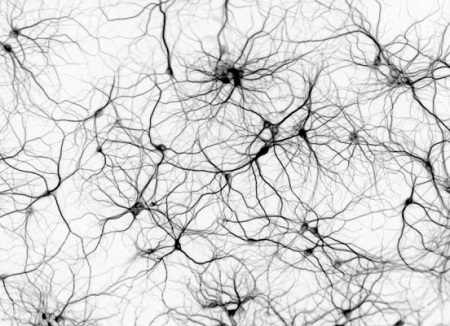
\includegraphics[scale=1.0]{bab2/gambar/jaringansaraf.jpg}}
    \end{center}
    \vspace{-20pt}
    \captionsetup{labelfont=bf, textfont=bf}
    \caption{Ilustrasi Jaringan Saraf Manusia}
    \vspace{-10pt}
    \captionsetup{labelfont=md, textfont=md}
    \caption*{Sumber: https://wccftech.com/scientists-artificial-neurons}
    % \caption*{Sumber: Zhang (2019)}
    \label{fig:jaringansaraf}
\end{figure}

Bentuk sel saraf sangat bervariasi dengan berbagai ukuran, bentuk, dan sifat elektrokimianya. Sebuah
sel saraf memiliki badan yang terdiri dari beberapa struktur penting meliputi \textit{soma},
\textit{dendrites}, \textit{axon}, dan \textit{synapses} seperti pada gambar~\ref{fig:selsaraf}.
Sebuah sel saraf akan menerima beberapa masukkan melalui \textit{synapses}, memproses inputan
tersebut melewati \textit{dendrites}, kemudian diteruskan melalui \textit{soma}, dan diberikan
kepada sel saraf lainnya melalui \textit{axon}~\cite{2019arXiv190601703Z}.

\begin{figure}[htbp]
    \begin{center}
        \fbox{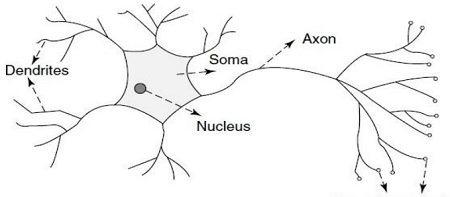
\includegraphics[scale=1.0]{bab2/gambar/selsaraf.jpg}}
    \end{center}
    \vspace{-20pt}
    \captionsetup{labelfont=bf, textfont=bf}
    \caption{Ilustrasi Sel Saraf Manusia}
    \vspace{-10pt}
    \captionsetup{labelfont=md, textfont=md}
    \caption*{Sumber: https://en.wikipedia.org/wiki/Neuron}
    % \caption*{Sumber: Zhang (2019)}
    \label{fig:selsaraf}
\end{figure}

\pagebreak

\section{Jaringan Saraf Tiruan}
\label{sec:2-JaringanSarafTiruan}

Jaringan Saraf Tiruan adalah sistem komputasi yang cara kerjanya menyerupai jaringan saraf pada otak
makhluk hidup. Sebuah jaringan saraf tiruan dapat dengan mandiri
memodelkan fungsi sembarang yang tingkat kesulitannya sesuai dengan jumlah koneksi yang tesedia.
Jarigan ini menyerupai jaringan saraf asli dimana
sebuah saraf tiruan menerima banyak masukkan dari saraf lainnya
kemudian dioperasikan dengan bobot yang terkadung pada sel tersebut dan akhirnya diteruskan ke sel
berikutnya~\cite{Sharma2012ACS}.

Sebuah sel saraf dapat dibagi menjadi empat bagian yang meliputi masukkan, bobot, fungsi
transfer atau aktivasi, dan keluaran. Jumlah masukkan pada suatu sel saraf tiruan berjumlah sebanyak
output dari sel-sel yang berada pada layer sebelumnya. Bobot sel adalah nilai numerik yang menjadi
identitas dari sel yang merupakan hasil penyesuaian dari proses latihan. Fungsi aktivasi adalah
sebuah fungsi menerima hasil operasi antara bobot dan masukkan. Keluaran merupakan hasil dari sel
yang diteruskan ke lapisan selanjutnya. Ilustrasi sebuah sel saraf tiruan dapat dilihat pada gambar
~\ref{fig:saraftiruan}~\cite{Sharma2012ACS}.

\begin{figure}[htbp]
    \begin{center}
        \fbox{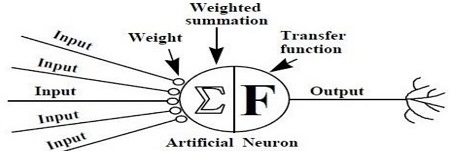
\includegraphics[scale=1.0]{bab2/gambar/saraftiruan.jpg}}
    \end{center}
    \vspace{-20pt}
    \captionsetup{labelfont=bf, textfont=bf}
    \caption{Ilustrasi Sel Saraf Tiruan}
    \vspace{-10pt}
    \captionsetup{labelfont=md, textfont=md}
    \caption*{Sumber: https://en.wikipedia.org/wiki/artificial\_neural\_network}
    % \caption*{Sumber: Zhang (2019)}
    \label{fig:saraftiruan}
\end{figure}

\pagebreak

\section{Fungsi Aktivasi}
\label{sec:2-FungsiAktivasi}

Fungsi aktivasi pada sel saraf tiruan berfungsi untuk mengkonversi hasil operasi matriks antara
masukkan dan bobot sebuah sel dari sistem linier menjadi sistem nonlinier. Konversi nilai ini dilakukan
agar setiap sel mengambil perannya pada saat proses pelatihan model. Beberapa fungsi aktivasi yang
dipakai pada umumnya adalah \textit{Sigmoid}, \textit{ReLU}, \textit{Tanh}, dan \textit{Softmax}
~\cite{2014arXiv1412.6830A}.

\textit{Rectified Linear Unit} adalah fungsi aktivasi yang paling umum digunakan dalam aplikasi
jaringan saraf tiruan. Fungsi aktivasi \textit{ReLU} membatasi nilai masukkannya dimana nilai yang
kurang dari nol akan diubah menjadi nol~\cite{Hinton_rectifiedlinear, 2018arXiv181103378N}.
Fungsi aktivasi \textit{Rectified Linear Unit} dapat dilihat pada persamaan 2.1 dengan grafik yang
dapat dilihat pada gambar~\ref{fig:relu}.

\begin{equation}
    \;f(x)=\;max\left(0,x\right)=\;\left\{\begin{array}{l}x_{i,\;}\;\;if\;x_i\;\geq\;0\\0,\;\;\;\;if\;x_i<\;0\;\;\end{array}\right.\;\;
\end{equation}

\begin{figure}[htbp]
    \begin{center}
        \fbox{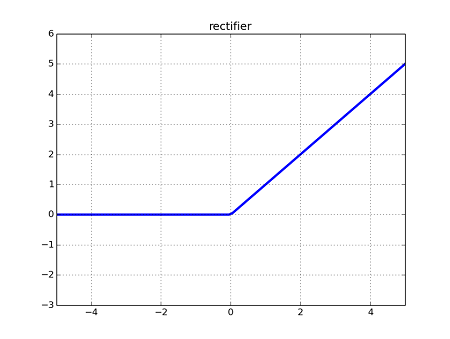
\includegraphics[scale=1.0]{bab2/gambar/relu.png}}
    \end{center}
    \vspace{-20pt}
    \captionsetup{labelfont=bf, textfont=bf}
    \caption{\textit{Rectified Linear Unit}}
    \vspace{-10pt}
    \captionsetup{labelfont=md, textfont=md}
    \caption*{Sumber: https://static.packt-cdn.com/products/graphics/B05478\_03\_11.png}
    % \caption*{Sumber: Zhang (2019)}
    \label{fig:relu}
\end{figure}

\section{\textit{Residual Network}}
\label{sec:2-ResidualNetwork}

\textit{Residual Network} atau \textit{ResNet} merupakan model jaringan saraf tiruan yang menggunakan \textit{residual block}
sebagai dasar dari setiap lapisan. Sebuah \textit{residual block} merupakan sebuah arsitektur jaringan
saraf tiruan kecil yang terdiri dari beberapa lapisan. Setiap blok akan menjumlahkan masukkan dan
keluarannya sehingga layer di dalam suatu blok hanya menambahkan pola-pola yang dipelajari.

Hal ini
memungkinkan \textit{ResNet} untuk memiliki jumlah blok yang sangat banyak sehingga dapat memetakan
suatu fungsi sembarang yang sulit sesuai dengan teorema penaksiran universal~\cite{2015arXiv151203385H}.
Jenis-jenis \textit{residual block} dapat dilihat pada gambar~\ref{fig:resblock}.

\begin{figure}[htbp]
    \begin{center}
        \fbox{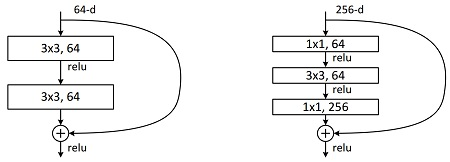
\includegraphics[scale=1.0]{bab2/gambar/resnet.jpg}}
    \end{center}
    \vspace{-20pt}
    \captionsetup{labelfont=bf, textfont=bf}
    \caption{\textit{Residual Block}}
    \vspace{-10pt}
    \captionsetup{labelfont=md, textfont=md}
    \caption*{Sumber: https://arxiv.org/abs/1512.03385}
    % \caption*{Sumber: Zhang (2019)}
    \label{fig:resblock}
\end{figure}

\section{Optimisasi Model}
\label{sec:2-OptimisasiModel}

Algoritma optimisasi model yang paling populer dalam melakukan pemelajaran model \textit{deep learning}
adalah \textit{gradient descent}. \textit{Gradient descent} meminimalisir selisih antara prediksi
model dan target sebenarnya dengan merubah bobot-bobot yang terdapat dalam model. Nilai bobot yang
ditambahkan berbanding terbalik dengan gradien hasil fungsi kesalahan terhadap masing-masing bobot.
Proses optimisasi dilakukan dengan melakukan \textit{backpropagation} yang
melibatkan beberapa elemen seperti \textit{learning rate},
dan \textit{loss function}. Tujuannya adalah untuk mencapai titik optimal pada sebuah bidang berdasarkan
hasil dari \textit{loss function}~\cite{2016arXiv160100013G}. Ilustrasi titik optimal digambarkan
pada gambar~\ref{fig:gradientdescent}.

\begin{figure}[htbp]
    \begin{center}
        \fbox{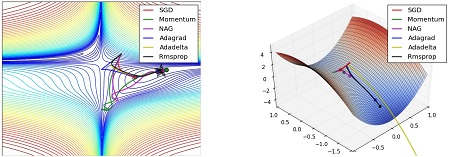
\includegraphics[scale=1.0]{bab2/gambar/gradientdescent.jpg}}
    \end{center}
    \vspace{-20pt}
    \captionsetup{labelfont=bf, textfont=bf}
    \caption{\textit{Gradient Descent}}
    \vspace{-10pt}
    \captionsetup{labelfont=md, textfont=md}
    \caption*{Sumber: https://arxiv.org/abs/1601.00013}
    % \caption*{Sumber: Zhang (2019)}
    \label{fig:gradientdescent}
\end{figure}

\subsection{\textit{Backpropagation}}

\textit{Backpropagation} adalah sebuah prosedur pemelajaran jaringan saraf tiruan yang secara
berulang-ulang kali menyesuaikan bobot setiap sel hingga selisih antara keluaran dan target menjadi
lebih kecil. Algoritma ini merupakan mengorganisasikan sebuah model jaringan untuk secara mandiri
mencari titik optimal secara berkala. Optimisasi dilakukan dengan melakukan \textit{forward-pass}
pada satu atau sebagian atau semua data yang ada ke dalam model untuk mendapatkan hasil prediksi.
Hasil tersebut kemudian diukur selisihnya dengan target yang sebenarnya menggunakan sebuah fungsi
kesalahan. Turuan parsial masing-masing bobot terhadap selisih kesalahan ini adalah kuantitas negatif
yang harus ditambahkan bobot yang berkaitan~\cite{Rumelhart:1986we}. Skema algoritma \textit{backpropagation}
dapat dilihat pada gambar~\ref{fig:backprop}.

\begin{figure}[htbp]
    \begin{center}
        \fbox{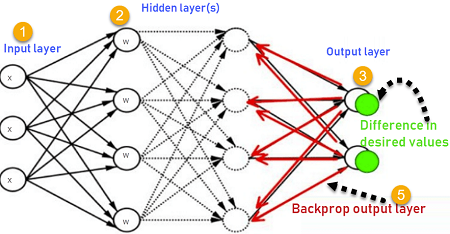
\includegraphics[scale=1.0]{bab2/gambar/backprop.png}}
    \end{center}
    \vspace{-20pt}
    \captionsetup{labelfont=bf, textfont=bf}
    \caption{Skema \textit{Backpropagation}}
    \vspace{-10pt}
    \captionsetup{labelfont=md, textfont=md}
    \caption*{Sumber: https://www.nature.com/articles/323533a0}
    % \caption*{Sumber: Zhang (2019)}
    \label{fig:backprop}
\end{figure}

\pagebreak

\subsection{\textit{Learning Rate}}

\textit{Learning rate} adalah sebuah nilai skalar yang menentukan seberapa besar sebuah bobot pada
jaringan saraf akan ditambahkan. Nilai \textit{learning rate} umumnya bernilai kecil karena
besar turunan parsial pada setiap iterasi akan berubah-ubah. Nilai \textit{learning rate} yang besar
akan merubah bobot dengan skala yang besar sehingga akurasi model cederung tidak stabil. Nilai
\textit{learning rate} yang kecil akan menghasilkan model yang stabil tetapi memerlukan jumlah iterasi
yang banyak seperti pada gambar~\ref{fig:lr}~\cite{2019arXiv190801878Y}.

\begin{figure}[htbp]
    \begin{center}
        \fbox{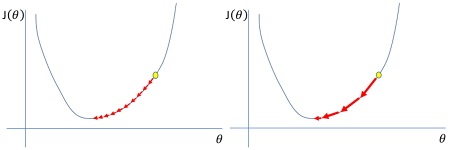
\includegraphics[scale=1.0]{bab2/gambar/lr.jpg}}
    \end{center}
    \vspace{-20pt}
    \captionsetup{labelfont=bf, textfont=bf}
    \caption{Ilustrasi Perbedaan \textit{Learning Rate}}
    \vspace{-10pt}
    \captionsetup{labelfont=md, textfont=md}
    \caption*{Sumber: https://arxiv.org/abs/1908.01878}
    % \caption*{Sumber: Zhang (2019)}
    \label{fig:lr}
\end{figure}

\subsection{\textit{Mean Squared Error}}
\textit{Mean squared error} adalah sebuah persamaan estimasi kesalahan dengan merata-ratakan
hasil dari pangkat dua selisih antara dua vektor. Fungsi kesalahan ini dipakai untuk mengukur
kesalahan model regresi dimana keluaran yang diukur bersifat kontinu. Persamaan ini akan selalu
bernilai positif dan nilai yang mendekati nol menandakan bahwa selisih antara dua vektor semakin kecil
seperti pada persamaan 2.2~\cite{TORABI201376}.

\begin{equation}
    MSE = \frac{1}{n}\Sigma_{i=1}^{n}{\Big(\frac{d_i -f_i}{\sigma_i}\Big)^2}
\end{equation}

\section{Estimasi Pose Dua Dimensi}
\label{sec:2-EstimasiPoseDuaDimensi}

Estimasi pose dua dimensi melakukan lokalisasi titik kunci anatomi atau bagian tubuh manusia
berdasarkan fungsi dari bagian tersebut pada sebuah gambar dua dimensi.
Setiap gambar unik dapat berisi jumlah orang
yang berbeda dan dapat muncul dengan posisi dan ukuran yang berbeda-beda. Interaksi antara manusia
dengan benda disekitarnya dapat menyebabkan oklusi dan hilangnya titik kunci anatomi yang dicari.
Kompleksitas permasalahan ini juga semakin meningkat berbanding lurus dengan jumlah orang yang ada
dalam suatu gambar~\cite{psfor}~\cite{kposolet}.

Pendekatan yang umum dilakukan adalah dengan mendeteksi setiap orang dalam setiap gambar secara
individu. Hal pertama yang dideteksi adalah lokalisasi kemunculan suatu benda yang dianggap sebagai
objek manusia dan kemudian mencari titik kunci anatomi dari objek tersebut.
Pendekatan \textit{top-down} seperti ini cocok dipakai untuk mendapatkan
\textit{single-person} dengan mudah tetapi kompleksitas yang proporsional dengan jumlah orang.
Sebaliknya dengan pendekatan \textit{bottom-up} dimana deteksi dilakukan dengan mencari alamat piksel
pada gambar yang dianggap adalah titik kunci anatomi dan dilanjutkan dengan membangun pose manusia
dari kandidat yang ada. Pendekatan \textit{bottom-up} cocok untuk menyelesaikan masalah
\textit{multi-person} dikarenakan pencarian kandidat titik kunci dapat dilakukan terlebih dahulu tanpa
harus mengetahui jumlah orang. Perbedaan pendekatan \textit{top-down} dan \textit{bottom-up}
dapat dilihat pada gambar~\ref{fig:tdbu}~\cite{8765346}.

\begin{figure}[htbp]
    \begin{center}
        \fbox{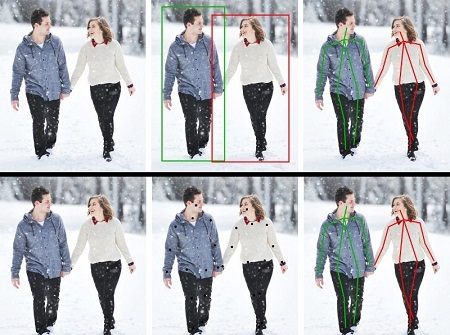
\includegraphics[scale=1.0]{bab2/gambar/tdbu.jpg}}
    \end{center}
    \vspace{-20pt}
    \captionsetup{labelfont=bf, textfont=bf}
    \caption{Pendekatan \textit{Top-Down} dan \textit{Bottom-Up}}
    \vspace{-10pt}
    \captionsetup{labelfont=md, textfont=md}
    \caption*{Sumber: https://mc.ai/an-overview-of-human-pose-estimation-with-deep-learning}
    % \caption*{Sumber: Zhang (2019)}
    \label{fig:tdbu}
\end{figure}

\section{Estimasi Pose Tiga Dimensi}
\label{sec:2-EstimasiPoseTigaDimensi}

Algoritma estimasi pose tiga dimensi merekonstruksi titik kunci tiga dimensi tubuh manusia dari
sebuah gambar dua dimensi. Proses pencarian titik kunci dibagi menjadi dua golongan yaitu pencarian
secara langsung menggunakan gambar sebagai masukkan dan pencarian bertahap dengan mencari titik kunci
anatomi dua dimensi terlebih dahulu kemudian dilanjutkan dengan pencarian titik kunci tiga dimensi.
Titik kunci yang didapatkan dapat berada dalam koordinat lokal dan global.
Pencarian secara langsung tidak menghasilkan akurasi yang tinggi dan cenderung buruk dalam mendeteksi
orientasi yang benar~\cite{2020arXiv200210322C}.

Titik kunci tiga dimensi yang berada dalam koordinat lokal menjadikan posisi pinggang sebagai titik
nol yang berarti lokasi pinggang akan selalu bernilai $\vec{hip} = [0.0, 0.0, 0.0]$. Posisi titik
kunci lain relatif terhadap titik pinggang. Hal ini menyebabkan pose yang ditangkap hanya bersifat
lokal yang berarti hanya memiliki satu orientasi lokal. Pencarian pose tiga dimensi lokal dari gambar
dua dimensi diilustrasikan pada gambar~\ref{fig:lokal}~\cite{martinez_2017_3dbaseline}.

\begin{figure}[htbp]
    \begin{center}
        \fbox{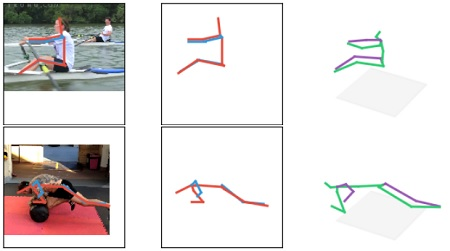
\includegraphics[scale=1.0]{bab2/gambar/lokal.jpg}}
    \end{center}
    \vspace{-20pt}
    \captionsetup{labelfont=bf, textfont=bf}
    \caption{Pencarian Pose Tiga Dimensi Lokal}
    \vspace{-10pt}
    \captionsetup{labelfont=md, textfont=md}
    \caption*{Sumber: https://arxiv.org/abs/1705.03098}
    % \caption*{Sumber: Zhang (2019)}
    \label{fig:lokal}
\end{figure}

Titik kunci tiga dimensi dapat juga berada dalam koordinat global yang berarti orientasi kamera
saat mengambil gambar diperhitungkan sebagai sebuah observasi virtual. Kompleksitas yang dihadapi
berkaitan dengan orientasi kamera yang berubah. Estimasi pose tiga dimensi global umumnya dilakukan
dengan mendeteksi titik kunci anatomi tubuh manusia ke dalam suatu dunia virtual tiga dimensi sehingga
dapat diamati dari berbagai sudut yang berkorelasi dengan kamera~\cite{2017arXiv170402447Z, 2019arXiv190700837M}.
Pencarian pose tiga dimensi global dari gambar dua dimensi diilustrasikan pada gambar~\ref{fig:global}.

\begin{figure}[htbp]
    \begin{center}
        \fbox{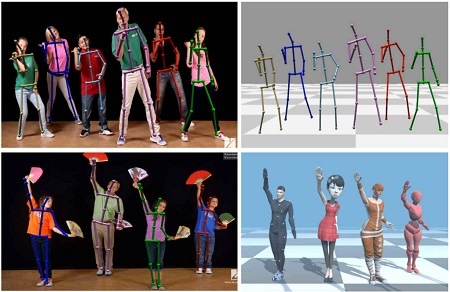
\includegraphics[scale=1.0]{bab2/gambar/global.jpg}}
    \end{center}
    \vspace{-20pt}
    \captionsetup{labelfont=bf, textfont=bf}
    \caption{Pencarian Pose Tiga Dimensi Global}
    \vspace{-10pt}
    \captionsetup{labelfont=md, textfont=md}
    \caption*{Sumber: http://gvv.mpi-inf.mpg.de/projects/SingleShotMultiPerson}
    % \caption*{Sumber: Zhang (2019)}
    \label{fig:global}
\end{figure}

\section{PyTorch}
\label{sec:2-PyTorch}

PyTorch merupakan \textit{framework} untuk melakukan \textit{deep learning} dengan bahasa pemrograman
python. Penggiat data umumnya menggunakan bahasa pemrograman ini dalam melakukan
riset pemanfaatan dan pengolahan data. PyTorch menyediakan implementasi grafik jaringan saraf tiruan yang bersifat dinamis.
Hal ini memungkinkan pengguna untuk mengubah arsitektur model secara cepat dalam setiap iterasi~\cite{2019arXiv191201703P}.


\section{\textit{Unified Modeling Language}}
\label{sec:2-uml}

\textit{Unified Modeling Language} (UML) merupakan bahasa pemodelan standar yang memiliki sintaks
dan semantik. UML bukan hanya sekedar diagram, tetapi juga menceritakan konteksnya. UML
diaplikasikan dengan beberapa maksud seperti percangan perangkat lunak, sarana komunikasi antara
perangkat lunak dengan proses bisnis, penjabaran sistem secara rinci dan pendokumentasian sistem
yang ada.

Para pengembang sistem berorientasi objek menggunakan bahasa model untuk menggambarkan, membangun
dan mendokumentasikan sistem yang mereka rancang. UML memungkinkan para pengembang aplikasi untuk
bekerja sama dengan bahasa model yang sama dalam mengaplikasikan beragam sistem. UML merupakan Alat
komunikasi yang konsisten dalam mendukung para pengembang saat ini. UML menyediakan sembilan jenis
diagram yaitu : \textit{Class Diagram, Packet Diagram, Use Case Diagram, Sequence Diagram,
    Communication Diagram, Statechart Diagram, Activity Diagram, Component Diagram} dan
\textit{Deployment Diagram}.

\textit{Activity Diagram} merupakan penggabungan dari berbagai alur aktivitas dalam sistem yang sedang
dirancang, bagaimana masing-masing alur berawal, \textit{decision} yang  mungkin  terjadi dan bagaimana
mereka  berakhir. \textit{Activity Diagram} juga dapat menggambarkan proses paralel yang mungkin terjadi
pada beberapa  eksekusi.


\begin{table}[htbp]
    \captionsetup{labelfont=bf, textfont=bf}
    \caption{Simbol-Simbol \textit{Activity Diagram}}
    \label{tab:simbolactdiagram}
    \vspace{-20pt}
    \begin{center}
        \begin{tabular}{|c|c|c|c| }
            \hline
            No & Nama                       & Gambar           & Keterangan                                \\ \hline

            1. & \begin{minipage}{.1\textwidth}
                
\includegraphics[width=\linewidth]{bab2/gambar/uml/initial.jpg}
            \end{minipage} & \textit{Initial} & Bagaimana  objek  dibentuk  atau diawali. \\ \hline

            2. & \begin{minipage}{.1\textwidth}
                
\includegraphics[width=\linewidth]{bab2/gambar/uml/final.jpg}
            \end{minipage} & \textit{Final}   & Bagaimana  objek dihancurkan.             \\ \hline

            3. & \begin{minipage}{.2\textwidth}
                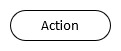
\includegraphics[width=\linewidth]{bab2/gambar/uml/action.jpg}
            \end{minipage} & \textit{Action}  & State eksekusi dari suatu aksi.           \\ \hline

            4. & \begin{minipage}{.2\textwidth}
                
\includegraphics[width=\linewidth]{bab2/gambar/uml/fork.jpg}
            \end{minipage} & \textit{Fork}    & Penggabungan atau pemisahan alur.         \\ \hline

            5. & \begin{minipage}{.2\textwidth}
                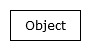
\includegraphics[width=\linewidth]{bab2/gambar/uml/object.jpg}
            \end{minipage} & \textit{Object}  & State hasil dari suatu aksi.              \\ \hline

            6. & \begin{minipage}{.2\textwidth}
                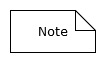
\includegraphics[width=\linewidth]{bab2/gambar/uml/note.jpg}
            \end{minipage} & \textit{Note}    & Keterangan tambahan suatu komponen.       \\ \hline
        \end{tabular}
    \end{center}
\end{table} %Bab 2.Tinjauan Pustaka


\chapter{METODOLOGI PENELITIAN}
\label{cha:3-MetodologiPenelitian}

\section{Gambaran Umum} \label{sec:3-GambaranUmum}

Penelitian ini membahas pemanfaatan data gambar sebagai acuan dalam melakukan pemelajaran dan
implementasi model \textit{deep neural network} untuk mencari dan memetakan koordinat tiga dimensi
pose tubuh manusia dalam sebuah rangkaian gambar secara lokal. Pengerjaan aplikasi mengutamakan dua
langkah penting yang meliputi pengolahan data dan pembuatan model. Aplikasi yang dibuat dapat menampilkan
plot grafik tiga dimensi menyerupai struktur anatomi tubuh manusia sesuai dengan pose hasil
estimasi dari gambar masukkan. Hasil pemelajaran model ditampilkan dalam grafik dua dimensi untuk
analisis lebih lanjut.

\textit{Dataset} yang digunakan dalam penelitian ini terbagi menjadi dua jenis yang meliputi
\textit{dataset} pemelajaran model dan \textit{dataset} inferensi aplikasi.
\textit{Dataset} pemelajaran model dikategorikan menjadi data pelatihan model dan data validasi model.
\textit{Dataset} pemelajaran model berisi gambar dan target posisi titik kunci anatomi dalam jumlah besar.
Data pelatihan model adalah data yang digunakan dalam proses pelatihan sebagai sampel bagi \textit{deep neural network}.
Data validasi model adalah data yang digunakan untuk menguji kebenaran fungsionalitas pemetaan yang
dipelajari saat pelatihan model. \textit{Dataset} inferensi aplikasi adalah data uji coba berbentuk
video tanpa target titik kunci yang digunakan untuk estimasi pose tubuh manusia secara sekuensial.

Pemelajaran model \textit{deep neural network} diimplementasikan menggunakan \textit{framework} PyTorch.
Kedua \textit{dataset} yang digunakan diolah terlebih dahulu sehingga memenuhi syarat PyTorch dalam melakukan
\textit{deep learning}.
Setiap model kemudian digunakan terhadap \textit{dataset} inferensi
aplikasi. Proses dan hasil estimasi diurai lebih lanjut dalam bentuk grafik visual.

\section{Kerangka Penelitian} \label{sec:3-KerangkaPenelitian}

Kerangka penelitian yang jelas dibutuhkan untuk memudahkan proses penelitian sehingga dapat
mempersingkat waktu pengerjaan. Proses penelitian dibagi menjadi tiga tahapan besar yang meliputi
tahap praproduksi, tahap produksi, dan tahap uji coba. Setiap tahapan tersebut dikerjakan secara
terurut dan sistematis. Alur setiap tahap diilustrasikan pada gambar~\ref{fig:kerangkapenelitian}.

\begin{figure}[htbp]
    \begin{center}
        \fbox{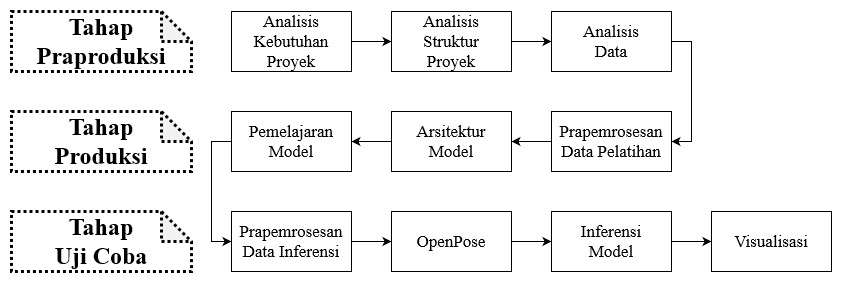
\includegraphics[width=11.9cm]{bab3/gambar/kerangka_penelitian.jpg}}
    \end{center}
    \vspace{-20pt}
    \captionsetup{labelfont=bf, textfont=bf}
    \caption{Kerangka Penelitian}
    \vspace{-10pt}
    \captionsetup{labelfont=md, textfont=md}
    % \caption*{Sumber: sumber}
    % \caption*{Sumber: nama(2019)}
    \label{fig:kerangkapenelitian}
\end{figure}

\section{Tahap Praproduksi} \label{sec:3-TahapPraproduksi}

Tahap praproduksi berisi langkah-langkah analisis yang menentukan alur pada tahap selanjutnya. Tahap
praproduksi dibagi menjadi beberapa langkah yang meliputi analisis kebutuhan proyek, analisis
struktur proyek, dan analisis data. Tahap ini menganalisis bagian-bagian pokok yang diperlukan
sehingga mengetahui langkah-langkah yang akan dilakukan pada tahap produksi.

\subsection{Analisis Kebutuhan Proyek}

Pemelajaran dan implementasi model ini memerlukan alat-alat pendukung berupa perangkat keras dan
perangkat lunak yang mencukupi. Spesifikasi perangkat keras dan perangkat lunak yang lebih besar
akan mempercepat proses pemelajaran model jaringan saraf tiruan.
Spesifikasi perangkat keras yang digunakan dalam penelitian ini
dapat dilihat pada tabel~\ref{tab:spesifikasiperangkatkeras}. Spesifikasi perangkat lunak yang
digunakan dalam penelitian ini dapat dilihat pada tabel~\ref{tab:spesifikasiperangkatlunak}.


\begin{table}[htbp]
    \captionsetup{labelfont=bf, textfont=bf}
    \caption{Spesifikasi Perangkat Keras}
    \label{tab:spesifikasiperangkatkeras}
    \vspace{-20pt}
    \begin{center}
        \begin{tabular}{|c|c|}
            \hline
            \multicolumn{2}{|c|}{\textbf{Perangkat Keras (Laptop)}} \\ \hline
            CPU & Intel Core I7 7700 HQ                             \\ \hline
            GPU & NVIDIA GTX 1060 6 GB                              \\ \hline
            RAM & 24 GB DDR4                                        \\ \hline
            SSD & NVME SAMSUNG 120 GB                               \\ \hline
            HDD & SATA 1 TB                                         \\ \hline
            % \multicolumn{1}{|c|}{RDF-3X}    & a & b & c & d & e & f & g \\ \hline
        \end{tabular}
    \end{center}
\end{table}

\begin{table}[htbp]
    \captionsetup{labelfont=bf, textfont=bf}
    \caption{Spesifikasi Perangkat Lunak}
    \label{tab:spesifikasiperangkatlunak}
    \vspace{-20pt}
    \begin{center}
        \begin{tabular}{|c|c|}
            \hline
            \multicolumn{2}{|c|}{\textbf{Perangkat Lunak}} \\ \hline
            Sistem Operasi      & Ubuntu 19.10             \\ \hline
            IDE                 & Jupyter Lab              \\ \hline
            Bahasa Pemrograman  & Python 3.7               \\ \hline
            \textit{Framework } & PyTorch 1.4              \\ \hline
        \end{tabular}
    \end{center}
\end{table}

\subsection{Analisis Struktur Proyek}

Perancangan struktur proyek yang sistematis diperlukan untuk meminimalisir kompleksitas dalam
melakukan pembuatan dan pemelajaran model. \textit{Integrated development environment} Jupyter Lab
memudahkan eksekusi perintah dengan sintaks bahasa pemrograman Python dalam bentuk sel interaktif
dalam berkas berekstensi ipynb. Setiap sel terdiri dari
\textit{input} dan \textit{output}. \textit{Input} berisi perintah yang akan dieksekusi, sedangkan
\textit{output} berisi hasil eksekusi yang dapat berupa teks ataupun grafik. Tampilan Jupyter Lab
dapat dilihat pada gambar~\ref{fig:jupyterlab}.

\begin{figure}[htbp]
    \begin{center}
        \fbox{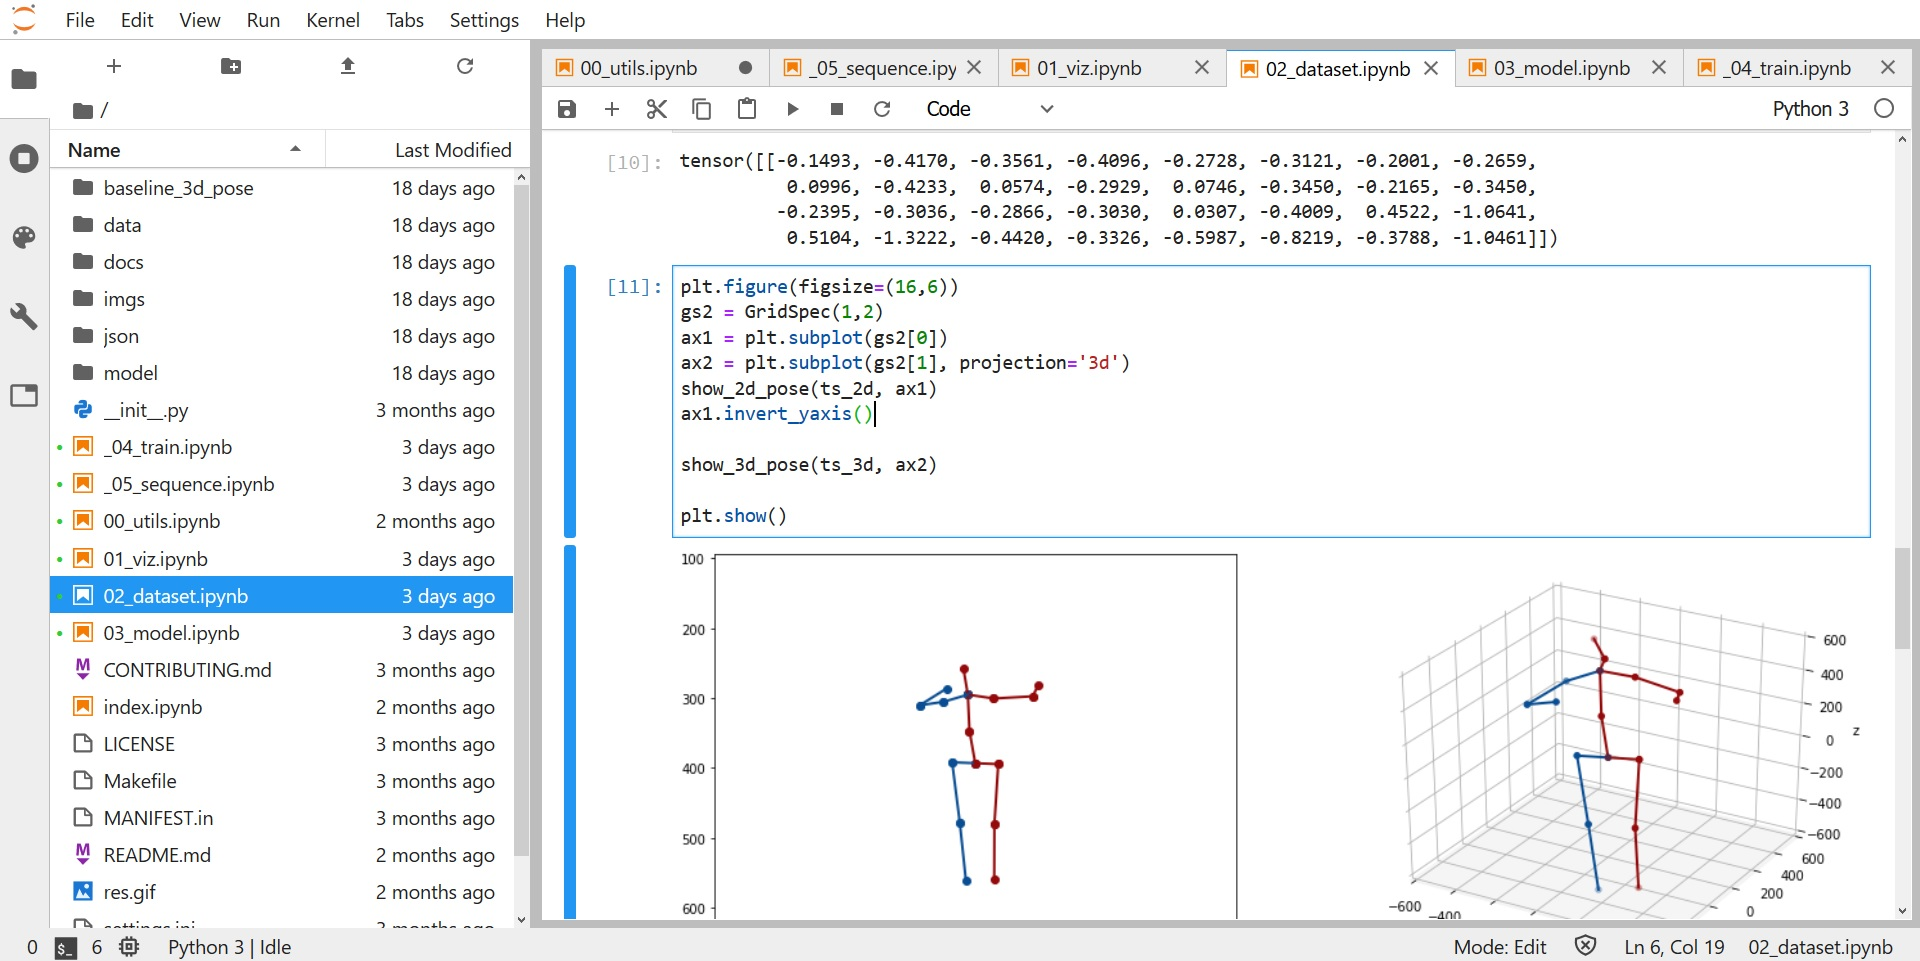
\includegraphics[width=11.9cm]{bab3/gambar/jupyterlab.jpg}}
    \end{center}
    \vspace{-20pt}
    \captionsetup{labelfont=bf, textfont=bf}
    \caption{Jupyter Lab}
    \vspace{-10pt}
    \captionsetup{labelfont=md, textfont=md}
    % \caption*{Sumber: sumber}
    % \caption*{Sumber: nama(2019)}
    \label{fig:jupyterlab}
\end{figure}


Struktur direktori yang disusun terdiri dari empat folder dan enam berkas \textit{interactive python notebook}
berekstensi ipynb. Folder data berisi data latihan model seperti pada gambar~\ref{fig:strukturdirektori}.
Folder imgs berisi rangkaian gambar yang
diambil dari rekaman video. Folder json menampung berkas yang berisi informasi titik kunci dua dimensi saat
inferensi. Folder model berisi \textit{checkpoint} model selama pelatihan.

Berkas berekstensi ipynb berisi kode pemrograman yang dibagi menjadi enam modul.
Berkas 00\_utils merupakan modul utilitas yang memudahkan proses memuat data, menampilkan data, menyimpan data, dan memanipulasi data.
Berkas 01\_viz adalah modul percobaan menampilkan data pelatihan dan data inferensi.
Berkas 03\_model merupakan modul pendefinisian arsitektur model.
Berkas 04\_train adalah modul pelatihan model.
Berkas 05\_sequence adalah modul percobaan inferensi model terhadap rangkaian gambar.

\begin{figure}[htbp]
    \begin{center}
        \fbox{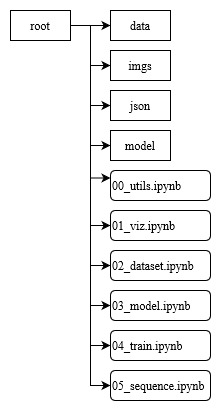
\includegraphics[height=11cm, width=11.9cm]{bab3/gambar/struktur_direktori.jpg}}
    \end{center}
    \vspace{-20pt}
    \captionsetup{labelfont=bf, textfont=bf}
    \caption{Struktur Direktori}
    \vspace{-10pt}
    \captionsetup{labelfont=md, textfont=md}
    % \caption*{Sumber: sumber}
    % \caption*{Sumber: nama(2019)}
    \label{fig:strukturdirektori}
\end{figure}


\subsection{Analisis Data}

Data pembuatan model yang digunakan adalah data pemetaan dari pose dua dimensi ke pose tiga dimensi.
Pose dua dimensi merupakan sampel, sedangkan pose tiga dimensi merupakan target. Sumber data adalah
Human3.6M Dataset mengenai informasi perakaman gerakan pose manusia yang menyimpan gambar dari
beberapa sisi beserta dengan pose dua dimensi dan tiga dimensinya. Informasi kedua pose tersebut
kemudian dipisah dan disimpan dalam file berekstensi "pt"~\cite{h36m_pami}.
Informasi mengenai data pemelajaran dapat dilihat pada tabel~\ref{tab:datapelatihanmodel}.
\begin{table}[htbp]
    \captionsetup{labelfont=bf, textfont=bf}
    \caption{Data Pemelajaran Model}
    \label{tab:datapelatihanmodel}
    \vspace{-20pt}
    \begin{center}
        \begin{tabular}{|c|c|}
            \hline
            Nama Berkas  & Isi                                                                                 \\ \hline
            rcams.pt     & matriks kamera \textit{motion capture} terhadap kamera perekam                      \\ \hline
            stat\_2d.pt  & \textit{mean}, \textit{standard-deviation}, dan \textit{skeleton} pose dua dimensi  \\ \hline
            stat\_3d.pt  & \textit{mean}, \textit{standard-deviation}, dan \textit{skeleton} pose tiga dimensi \\ \hline
            test\_2d.pt  & data pose dua dimensi untuk validasi model                                          \\ \hline
            test\_3d.pt  & data pose tiga dimensi untuk validasi model                                         \\ \hline
            train\_2d.pt & data pose dua dimensi untuk pelatihan model                                         \\ \hline
            train\_3d.pt & data pose tiga dimensi untuk pelatihan model                                        \\ \hline
        \end{tabular}
    \end{center}
    \vspace{-10pt}
\end{table}

Data inferensi model yang digunakan berupa video yang direkam menggunakan kamera diatas sebuah
\textit{tripod}. Hasil rekaman berupa sebuah video monokuler berisi seorang aktor yang memperagakan
berbagai pose dasar. Pose-pose yang diperagakan mencakupi gerakan lengan, gerakan kaki, gerakan pinggang,
gerakan kepala, dan gerakan memutar. Kompleksitas gerakan ini mengakibatkan terjadinya oklusi pada
beberapa bagian badan yang berarti suatu anggota badan menutupi anggota badan lainnya.

Kualitas perekaman video diturunkan dengan menggunakan pencahayaan yang satu arah.
Efek \textit{motion blur} diaktifkan sehingga gerakan yang cepat akan mengalami pengaburan.
Kompleksitas gambar juga ditingkatkan dengan
\textit{aspect ratio} yang bernilai 19 : 6 dengan tipe rekaman \textit{potrait} menyebabkan area rekaman
hanya berada ditengah dan diapit oleh area piksel hitam.
Beberapa \textit{frame} dari data inferensi model dapat dilihat pada gambar
~\ref{fig:frame00077},~\ref{fig:frame00173}, dan~\ref{fig:frame00232}.

\begin{figure}[htbp]
    \begin{center}
        \fbox{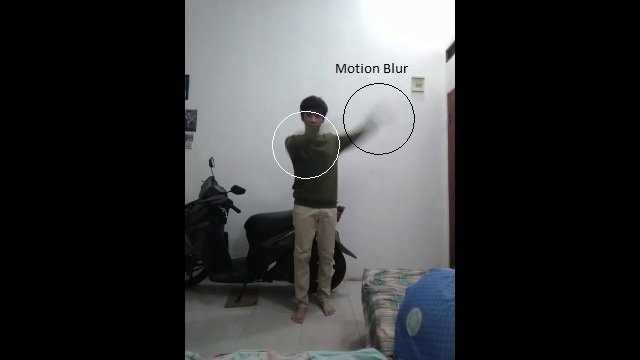
\includegraphics[width=11.9cm]{bab3/gambar/00077.jpg}}
    \end{center}
    \vspace{-20pt}
    \captionsetup{labelfont=bf, textfont=bf}
    \caption{\textit{Frame} 00077}
    \vspace{-10pt}
    \captionsetup{labelfont=md, textfont=md}
    % \caption*{Sumber: sumber}
    % \caption*{Sumber: nama(2019)}
    \label{fig:frame00077}
\end{figure}

\begin{figure}[htbp]
    \begin{center}
        \fbox{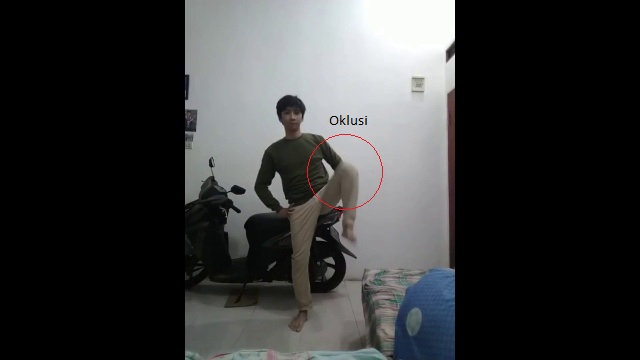
\includegraphics[width=11.9cm]{bab3/gambar/00173.jpg}}
    \end{center}
    \vspace{-20pt}
    \captionsetup{labelfont=bf, textfont=bf}
    \caption{\textit{Frame} 00173}
    \vspace{-10pt}
    \captionsetup{labelfont=md, textfont=md}
    % \caption*{Sumber: sumber}
    % \caption*{Sumber: nama(2019)}
    \label{fig:frame00173}
\end{figure}

\begin{figure}[htbp]
    \begin{center}
        \fbox{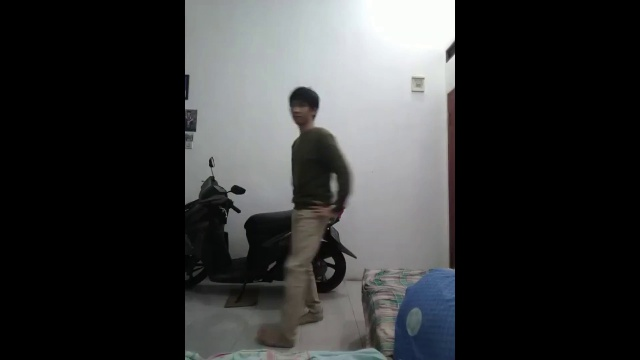
\includegraphics[width=11.9cm]{bab3/gambar/00232.jpg}}
    \end{center}
    \vspace{-20pt}
    \captionsetup{labelfont=bf, textfont=bf}
    \caption{\textit{Frame} 00232}
    \vspace{-10pt}
    \captionsetup{labelfont=md, textfont=md}
    % \caption*{Sumber: sumber}
    % \caption*{Sumber: nama(2019)}
    \label{fig:frame00232}
\end{figure}

\section{Tahap Produksi} \label{sec:3-TahapProduksi}

Tahap produksi merupakan tahap kedua yang dimana pengerjaan dilakukan. Tahap ini terdiri dari
tiga langkah utama yaitu prapemrosesan data pelatihan, pembuatan arsitektur model, dan pemelajaran model.


\subsection{Prapemrosesan Data Pelatihan}

\textit{Dataset} pembuatan model terbagi menjadi dua kategori yaitu data pelatihan
(train\_2d.pt dan train\_3d.pt) dan data validasi (test\_2d.pt dan test\_3d.pt) .
Kedua data ini memiliki struktur dan bentuk yang sama sehingga prapemrosesan yang dilakukan juga sama.
Setiap sampel pada data terdiri dari satu pose dua dimensi dan satu pose tiga dimensi.
Perbedaan daripada kedua data ini terletak pada jumlah sampelnya. Data pelatihan berisi sebanyak
1.559.752 pasang sampel sedangkan data validasi memiliki 550.644 pasang sampel.

Berkas test\_2d.pt, test\_3d.pt, train\_2d.pt, dan train\_3d.pt merupakan berkas hasil konversi
struktur data \textit{dictionary} yang telah berbentuk \textit{serialized}.
Struktur \textit{dictionary} yang berada didalam memori disimpan ke media SSD dalam bentuk \textit{byte stream}.
Berkas-berkas ini harus dibaca dengan mekanisme \textit{deserializing} yaitu membangun ulang sebuah
struktur data yang sama dengan membaca rangkaian \textit{byte} sehingga dapat digunakan pada proses pelatihan model.

Mekanisme pemuatan data dilakukan secara \textit{stochastic} dikarenakan hasil konversi data yang
berukuran sangat besar. Serangkaian pasangan kunci dan target diproses dengan ukuran tertentu
yang disebut dengan \textit{mini-batch} sehingga
VRAM pada GPU tidak mengalami \textit{overflow}. Pemuatan data secara \textit{stochastic} juga
mempercepat proses pelatihan model karena lebih sedikit data yang harus dikalkukasi sebelum melakukan
pemuktahiran.

Kelas Dataset dan DataLoader pada \textit{framework} PyTorch memiliki fungsionalitas untuk melakukan
pembacaan dan pembagian rangkaian data secara \textit{stochastic}. Kelas Dataset dapat membaca berkas
berekstensi "pt" dari media SSD kemudian dimuat kedalam memori. Kelas DataLoader dapat memindahkan
informasi didalam kelas Dataset ke VRAM pada GPU berbentuk \textit{mini-batch} sehingga dapat diproses secara
\textit{stochastic} dan paralel.

Prapemrosesan data pelatihan dan data validasi dilakukan dengan cara yang sama. Langkah pertama
yang dilakukan adalah melakukan cek apakah data yang diinginkan adalah data pelatihan atau data
validasi. Data tersebut kemudian dimuat dan disimpan kedalam memori. DataLoader menerima objek
tersebut kemudian melakukan pengacakan data dan pembagian \textit{mini-batch}. Hasil objek dapat
diiterasi untuk melakukan pelatihan model. Skema prapemrosesan data dapat dilihat pada gambar~\ref{fig:act_diagram}.

\begin{figure}[htbp]
    \begin{center}
        \fbox{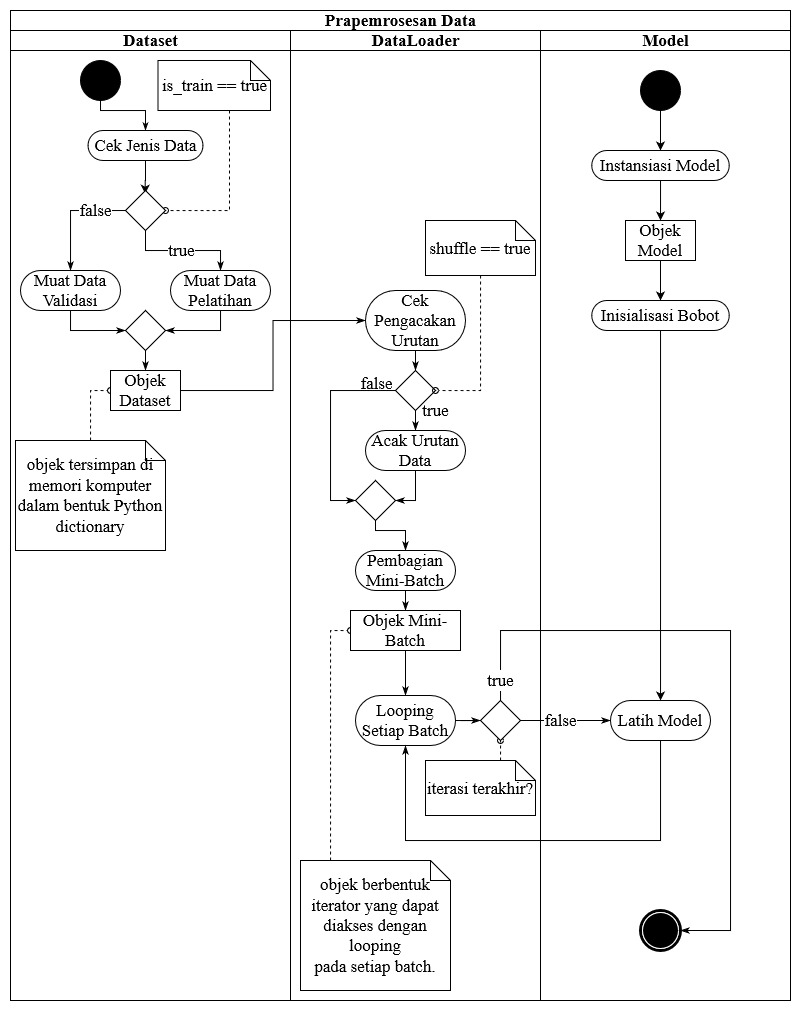
\includegraphics[width=11.9cm]{bab3/gambar/act_diagram.jpg}}
    \end{center}
    \vspace{-20pt}
    \captionsetup{labelfont=bf, textfont=bf}
    \caption{\textit{Activity Diagram} Prapemrosesan Data}
    \vspace{-10pt}
    \captionsetup{labelfont=md, textfont=md}
    % \caption*{Sumber: sumber}
    % \caption*{Sumber: nama(2019)}
    \label{fig:act_diagram}
\end{figure}

\subsection{Arsitektur Model}

Arsitektur model jaringan saraf tiruan yang digunakan memiliki \textit{input} berbentuk vektor dengan ukuran
tiga puluh dua dan \textit{output} berbentuk vektor dengan ukuran empat puluh delapan. Rangkaian lapisan yang
menghubungkan \textit{input} dan \textit{output} berupa lapisan \textit{residual network}. Bobot setiap
lapisan diinisialisasi secara acak dengan distribusi normal.

Sebuah lapisan \textit{residual network} merupakan jaringan dengan arsitektur kecil dan sederhana yang
dapat dipasang atau dibongkar secara modular yang disebut ResLinear. Lapisan ResLinear melakukan operasi
penjumlahan antara \textit{input} dan \textit{output}. Sebuah ResLinear memiliki dua
lapisan linier, dua lapisan \textit{Batchnorm}, dua lapisan \textit{Dropout}, dan dua lapisan \textit{ReLU}.
Komponen-komponen penyusun sebuah lapisan ResLinear dengan ukuran \textit{input a} dan ukuran \textit{output b} seperti
pada gambar~\ref{fig:reslinear}.

\begin{figure}[htbp]
    \begin{center}
        \fbox{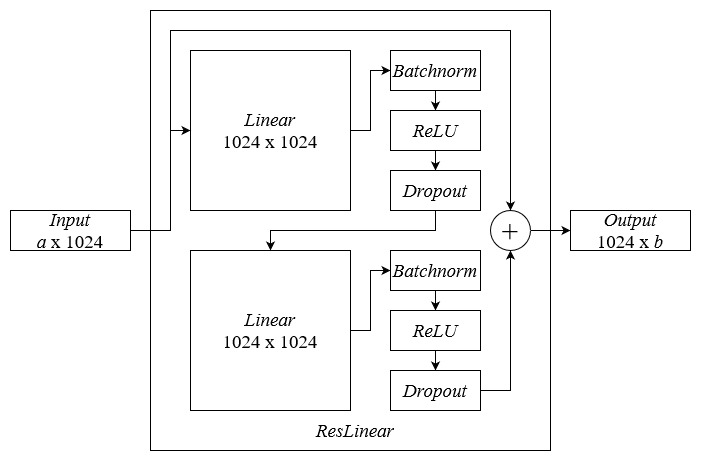
\includegraphics[width=11.9cm]{bab3/gambar/reslinear.jpg}}
    \end{center}
    \vspace{-20pt}
    \captionsetup{labelfont=bf, textfont=bf}
    \caption{Arsitektur Lapisan ResLinear}
    \vspace{-10pt}
    \captionsetup{labelfont=md, textfont=md}
    % \caption*{Sumber: sumber}
    % \caption*{Sumber: nama(2019)}
    \label{fig:reslinear}
\end{figure}

Arsitektur model secara keseluruhan terdiri dari tiga kelompok yang meliputi lapisan awal, lapisan
\textit{residual}, dan lapisan akhir. Lapisan awal menjembatani data \textit{input} dan lapisan \textit{residual}
dengan menggunakan sebuah lapisan linier sebagai penyambung. Lapisan \textit{residual} terdiri dari
dua buah lapisan ResLinear yang berfungsi untuk memetakan pola data \textit{input} terhadap data \textit{output}.
Lapisan akhir menjembatani hasil pemetaan yang dilakukan oleh lapisan \textit{residual} terhadap data \textit{output}.
Arsitektur model dapat dilihat pada gambar~\ref{fig:arsitektur}.

\begin{figure}[htbp]
    \begin{center}
        \fbox{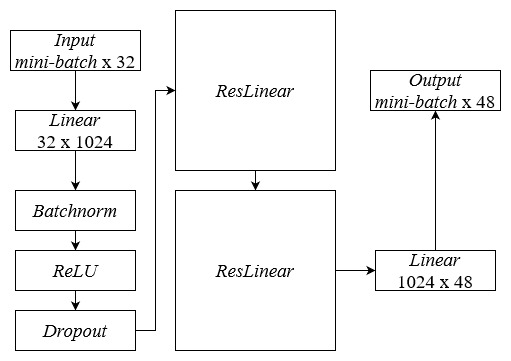
\includegraphics[width=11.9cm]{bab3/gambar/arsitektur.jpg}}
    \end{center}
    \vspace{-20pt}
    \captionsetup{labelfont=bf, textfont=bf}
    \caption{Arsitektur Model}
    \vspace{-10pt}
    \captionsetup{labelfont=md, textfont=md}
    % \caption*{Sumber: sumber}
    % \caption*{Sumber: nama(2019)}
    \label{fig:arsitektur}
\end{figure}

\subsection{Pemelajaran Model}

Pemelajaran model merupakan kelanjutan dari prapemrosesan data. Sebuah model baru diinstansiasii
sehingga menghasilkan objek model. Objek model tersebut kemudian menginisialisasi bobot parameter
dengan bilangan acak dari distribusi normal. \textit{Batch input} yang berasal dari interasi DataLoader
diproses oleh model dengan metode \textit{feed-forward}. Hasil prediksi sementara dari model
didapatkan yang kemudian dibandingkan tingkat kebenarannya menggunakan fungsi kesalahan.
Fungsi kesalahan \textit{mean squared error} menghasilkan angka kuantitas kesalahan. Angka ini merupakan
tolak ukur seberapa akurat kemampuan model dalam menghasilkan output yang relevan. Apabila model tidak
berada dalam status "is\_train", maka kuantitas kesalahan yang didapatkan langsung disimpan dalam bentuk
\textit{array} untuk keperluan analisis. Apabila model berada dalam status "is\_train", maka model
melakukan \textit{backpropagation} untuk menghasilkan gradien bobot. \textit{Learning rate} kemudian
dibagi dengan dua sehingga menjadi lebih kecil. Penyesuaian bobot dilakukan dengan menjumlahkan bobot
dengan hasil operasi perkalian antara \textit{learning rate} dan gradien bobot. Bobot model yang telah
diperbarui disimpan berserta dengan kuantitas kesalahannya. Algoritma yang sama akan diulangi pada setiap \textit{batch input}.
Skema pemelajaran model dapat dilihat pada gambar~\ref{fig:learning}.

\begin{figure}[htbp]
    \begin{center}
        \fbox{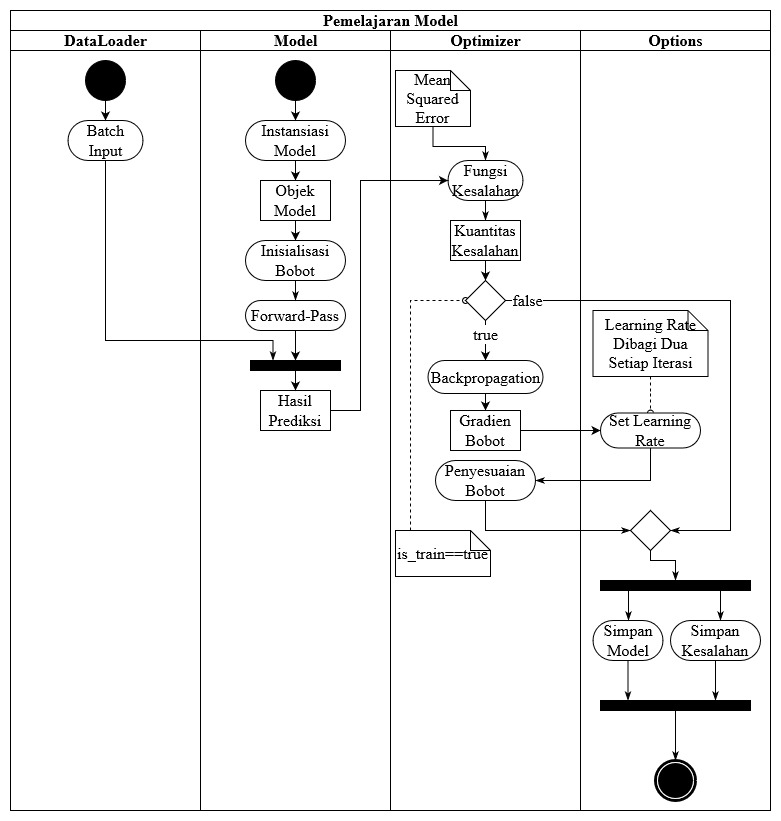
\includegraphics[width=11.9cm]{bab3/gambar/learning.jpg}}
    \end{center}
    \vspace{-20pt}
    \captionsetup{labelfont=bf, textfont=bf}
    \caption{\textit{Activity Diagram} Pemelajaran Model}
    \vspace{-10pt}
    \captionsetup{labelfont=md, textfont=md}
    % \caption*{Sumber: sumber}
    % \caption*{Sumber: nama(2019)}
    \label{fig:learning}
\end{figure}

\section{Tahap Uji Coba} \label{sec:3-TahapUjiCoba}

Tahap uji coba berisi langkah-langkah uji coba penggunaan model.
Tahap uji coba dibagi menjadi beberapa langkah yang meliputi prapemrosesan data inferensi,
penggunaan OpenPose, inferensi model, dan visualisasi. Tahap ini bertujuan untuk menggunakan model
sebagai aplikasi untuk mengestimasi pose tiga dimensi dari gambar monokuler.

\subsection{Prapemrosesan Data Inferensi}

\subsection{OpenPose}

\subsection{Inferensi Model}

\subsection{Visualisasi}

% \begin{table}[htbp]
%     \captionsetup{labelfont=bf, textfont=bf}
%     \caption{Sebuah tabel}
%     \vspace{-20pt}
%     \begin{center}
%         \begin{tabular}{| l c r |}
%             \hline
%             1 & 2 & 3 \\
%             4 & 5 & 6 \\
%             7 & 8 & 9 \\
%             \hline
%         \end{tabular}
%     \end{center}
%     \vspace{-10pt}
%     \captionsetup{labelfont=md, textfont=md}
%     % \caption*{Sumber: Bego Lu}
% \end{table} %Bab 3.Pendekatan


\chapter{PEMBUATAN DAN UJI COBA}
\label{cha:4-PembuatanDanUjiCoba}

\section{Persiapan pengujian}
\label{sec:4-PersiapanPengujian}

Berisi langkah2 untuk persiapan pengujian, bisa secara pembuktian secara teoritis, empiris, simulasi, dll.

\section{Pelaksanaan Pengujian}
\label{sec:4-PelaksanaanPengujian}

Berisi tentang langkah2 pelaksanaan

\section{Hasil dan Diskusi}
\label{sec:4-HasilDiskusi}

Berisi tentang hasil2 pengujian, ulasan diskusi dari penghasilan dan memberikan penekanan hal yang penting dari pengujian.
 %Bab 4.Hasil dan Analisis


\chapter{PENUTUP}
\label{cha:5-PENUTUP}

\section{Kesimpulan}
\label{sec:5-Kesimpulan}

Aplikasi estimasi pose tiga dimensi menggunakan model \textit{deep neural network} berhasil dilatih.
Model melakukan pemelajaran mandiri menggunakan pose dua dimensi sebagai \textit{input}
dan pose tiga dimensi sebagai \textit{output}.
Pengambilan data gambar monokuler dapat diperoleh dengan satu
lensa kamera saja, berbeda dengan konfigurasi \textit{motion capture}
yang memerlukan beberapa kamera untuk melakukan \textit{grounding}.
Model melakukan pemelajaran
selama sepuluh \textit{epochs} dengan hasil rata-rata kesalahan akhir bernilai 0.0584 pada data pelatihan
dan 0.0437 pada data validasi. Kesalahan tersebut mencakup 4.37 persen dari jumlah
data total yang gagal diestimasi secara lengkap.
Nilai kesalahan data pelatihan masih lebih besar daripada nilai data validasi.
Hal ini menandakan model masih berada pada kondisi \textit{underfitting} dimana selisih kedua nilai tersebut relatif
besar. Model yang lebih baik dapat didapatkan dengan melatih model dalam jumlah \textit{epochs} yang
lebih banyak dan berhenti saat mulai terjadi \textit{overfitting}.

\section{Saran}
\label{sec:5-Saran}

Pengembangan model \textit{deep neural network} ini masih menggunakan arsitektur minimalis, data dengan
satu domain, dan memiliki tahapan yang tidak efisien. Pengembangan selanjutnya disarankan menggunakan
arsitektur yang lebih efisien. Arsitekur \textit{residual network} merupakan arsitektur yang paling
bagus pada saat penulisan ini dilakukan. Estimasi pose tiga dimensi dapat dijadikan sebagai Aplikasi
pembaca pose manusia didalam berbagai bidang seperti pengganti motion capture, analisis kamera otomatis,
aplikasi medis, dan sebagainya.
Algoritma pemelajaran yang lebih efisien juga disarankan
pada penelitian mendatang. Data dengan domain yang lebih luas juga merupakan hal yang penting seperti
estimasi pose pada hewan tertentu. Dengan demikian penelitian ini dapat bermanfaat dan dapat dikembangkan
menjadi jauh lebih baik lagi pada masa mendatang. %Bab 5.Penutup

% diatas menunjukkan SubDir/nama file tex, bisa ditambah/dikurang sesuai kebutuhan

% # akhir bagian isi # ==================================================

% # mulai bagian Daftar Pustaka # ============================================
\newpage
\pagestyle{plain}
\addcontentsline{toc}{chapter}{DAFTAR PUSTAKA} %memasukkan daftar pustaka di daftar isi
\bibliographystyle{abbrv}
\bibliography{MainTemplateSkripsi} %file menyimpan bibtex

% # akhir bagian referensi # ============================================

\newpage
\pagestyle{plain}
\setcounter{page}{1} %mulai dari halaman L-1
\renewcommand{\thepage}{L\arabic{page}}
\newpage %lampiran
\addcontentsline{toc}{chapter}{LAMPIRAN}
\singlespacing
\begin{center}
    \begin{large}\textbf{LAMPIRAN}\\\end{large}
\end{center}
\vspace{5mm}

% \begin{multicols}{2}
% \small

\begin{lstlisting}[language=Python,multicols=2,basicstyle=\scriptsize\mdseries,breaklines=true]
    # Lampiran 1: Kelas Dataset
    class Human36Dataset(Dataset):
        def __init__(self, actions, data_path, is_train=True):
            self.actions, self.data_path, self.is_train = actions, data_path, is_train
            self.inp_list, self.out_list, self.key_list = [], [], []

            if self.is_train:
                self.data_2d = torch.load(data_path/'train_2d.pt')
                self.data_3d = torch.load(data_path/'train_3d.pt')
            else:
                self.data_2d = torch.load(data_path/'test_2d.pt')
                self.data_3d = torch.load(data_path/'test_3d.pt')

            for key in self.data_2d.keys():
                assert self.data_2d[key].shape[0] == self.data_3d[key].shape[0]
                num_file = self.data_2d[key].shape[0]
                for i in range(num_file):
                    self.inp_list.append(self.data_2d[key][i])
                    self.out_list.append(self.data_3d[key][i])
                    self.key_list.append(key)

        def __getitem__(self, idx):
            inp = torch.from_numpy(self.inp_list[idx]).float()
            out = torch.from_numpy(self.out_list[idx]).float()
            return inp, out

        def get_key(self, idx):
            return self.key_list[idx]

        def __len__(self):
            return len(self.inp_list)

    # Lampiran 2: Kelas ResLinear
    class ResLinear(nn.Module):
        def __init__(self, size, pd=0.5):
            super().__init__()
            self.size = size
            self.relu = nn.ReLU(inplace=True)
            self.drop = nn.Dropout(pd)
            # learnable
            self.ln1 = nn.Linear(self.size, self.size)
            self.bn2 = nn.BatchNorm1d(self.size)
            self.ln3 = nn.Linear(self.size, self.size)
            self.bn4 = nn.BatchNorm1d(self.size)
        def forward(self, x):
            y = self.drop(self.relu(self.bn2(self.ln1(x))))
            y = self.drop(self.relu(self.bn4(self.ln3(y))))
            return x + y

    # Lampiran 3: Arsitektur Model
    class Model(nn.Module):
        def __init__(self, size=1024, num_res_lyr=2, pd=0.5):
            super().__init__()
            self.size, self.num_res_lyr, self.pd = size, num_res_lyr, pd
            self.input_size, self.output_size = 32, 48
            self.relu = nn.ReLU(inplace=True)
            self.drop = nn.Dropout(self.pd)

            # input size
            self.ln_in = nn.Linear(self.input_size, self.size)
            self.bn_in = nn.BatchNorm1d(self.size)

            # res layers
            self.lins = []
            for i in range(num_res_lyr):
                self.lins.append(ResLinear(self.size, self.pd))
            self.lins = nn.ModuleList(self.lins)

            # output size
            self.ln_out = nn.Linear(self.size, self.output_size)
        def forward(self, x):
            y = self.drop(self.relu(self.bn_in(self.ln_in(x))))
            for i in range(self.num_res_lyr):
                y = self.lins[i](y)
            y = self.ln_out(y)
            return y

    # Lampiran 4: Options
    class Options():
        def __init__(self):
            # paths
            self.data_path = Path('data')
            self.model_path = Path('model')

            # train options
            self.actions = 'All'
            self.attempt_id = '01'
            self.attempt_path = Path('model')/self.attempt_id

            self.load_ckpt = False

            # train hyper-params
            self.bs = 128
            self.epochs = 10
            self.lr = 1e-3

            # model hyper-params
            self.size = 1024
            self.stages = 2
            self.dropout = 0.5

    # Lampiran 5: Pemuatan Data
    stat_3d = torch.load(data_path/'stat_3d.pt')
    stat_2d = torch.load(data_path/'stat_2d.pt')
    rcams = torch.load(data_path/'rcams.pt')

    mean_2d = stat_2d['mean']
    std_2d = stat_2d['std']
    dim_use_2d = stat_2d['dim_use']
    dim_ignore_2d = stat_2d['dim_ignore']

    mean_3d = stat_3d['mean']
    std_3d = stat_3d['std']
    dim_use_3d = stat_3d['dim_use']
    dim_ignore_3d = stat_3d['dim_ignore']

    # Lampiran 6: Instansiasi Dataset dan DataLoader
    train_ds = Human36Dataset(get_actions(options.actions), options.data_path, is_train=True)
    train_dl = DataLoader(train_ds, batch_size=options.bs, shuffle=True)
    test_ds = Human36Dataset(get_actions(options.actions), options.data_path, is_train=False)
    test_dl = DataLoader(test_ds, batch_size=options.bs, shuffle=False)

    # Lampiran 7: Algoritma Pelatihan
    def train(train_dl, model, criterion, optimizer, options, mb):
        model.train()
        loss_list = []
        skel_loss_list = []
        for xb, yb in progress_bar(train_dl, parent=mb):
            xb, yb = xb.cuda(), yb.cuda()
            yhat = model(xb)
            optimizer.zero_grad()
            loss_skel = criterion(yhat, yb)
            loss = loss_skel.mean()
            loss.backward()
            nn.utils.clip_grad_norm_(model.parameters(), max_norm=1)
            optimizer.step()

            loss_list.append(loss.item())
            skel_loss_list.append(loss_skel.data.cpu().numpy())

            mb.child.comment = f'train loss: {loss.item()}'
        return loss_list, skel_loss_list

    # Lampiran 8: Algoritma Validasi
    def test(test_dl, model, criterion, options, mb):
        model.eval()
        loss_list = []
        skel_loss_list = []
        for xb, yb in progress_bar(test_dl, parent=mb):
            xb, yb = xb.cuda(), yb.cuda()
            with torch.no_grad():
                yhat = model(xb)
                loss_skel = criterion(yhat, yb)
                loss = loss_skel.mean()
            loss_list.append(loss.item())
            skel_loss_list.append(loss_skel.data.cpu().numpy())
            mb.child.comment = f'test loss: {loss.item()}'
        return loss_list, skel_loss_list

    # Lampiran 9: Instansiasi Model
    model = Model()
    model = model.cuda()
    model.apply(init_kaiming)
    print(f'total params: {sum(p.numel() for p in model.parameters())}')

    criterion = nn.MSELoss(reduction='none').cuda()
    optimizer = optim.Adam(model.parameters(), lr=options.lr)

    if options.load_ckpt:
        options = torch.load('model/01/options.pt')
        model_state = torch.load(options.attempt_path/'last_model.pt')
        optimizer_state = torch.load(options.attempt_path/'last_optimizer.pt')
        model.load_state_dict(model_state)
        optimizer.load_state_dict(optimizer_state)

    # Lampiran 10: Visualisasi Titik Kunci
    key = train_key_list[184]
    plt.figure(figsize=(16,6))
    gs2 = GridSpec(1,2)
    ax1 = plt.subplot(gs2[0])
    ax2 = plt.subplot(gs2[1], projection='3d')

    idx = 200

    ts_2d = utils.unnormalize_data(train_set_2d[key][idx], mean_2d, std_2d, dim_ignore_2d)[0]

    ts_3d = utils.unnormalize_data(train_set_3d[key][idx], mean_3d, std_3d, dim_ignore_3d)[0]
    ts_3d = utils.cam_to_world_centered(ts_3d, key, rcams)

    utils.show_2d_pose(ts_2d, ax1)
    ax1.invert_yaxis()

    utils.show_3d_pose(ts_3d, ax2)

    plt.show()

    # Lampiran 11: Visualisasi Inferensi
    ## %matplotlib qt
    fig = plt.figure(figsize=(15,15))
    gs = GridSpec(2, 2)
    ax0 = plt.subplot(gs[0])
    ax1 = plt.subplot(gs[1])
    ax2 = plt.subplot(gs[2])
    ax3 = plt.subplot(gs[3], projection='3d')
    ax3.view_init(elev=20, azim=70)

    img0 = None
    img1 = None
    for i in range(len(img_lists)):
    # for i in range(3):
        if img0 is None:
            img0 = ax0.imshow(img_ls[i])
        else:
            img0.set_data(img_ls[i])

        if img1 is None:
            img1 = ax1.imshow(out_ls[i])
        else:
            img1.set_data(out_ls[i])

        ax2.clear()
        show_2d_pose(kp_ls[i], ax2)
        ax2.invert_yaxis()

        ax3.clear()
        show_3d_pose(kp3d_ls[i], ax3)

        plt.pause(1e-25)
        plt.draw()
        plt.savefig(f'imgs/asd/bro{i}.jpg')

    # Lampiran 12: Plot Grafik
    train_loss_lists = []
    train_mean = []
    train_max = []
    train_min = []
    for i in range(options.epochs):
        tll = torch.load(options.attempt_path/f'train_loss_list_e{i}.pt')
        train_mean.append(np.mean(tll))
        train_max.append(np.max(tll))
        train_min.append(np.min(tll))
        train_loss_lists.append(tll)
    test_loss_lists = []
    test_mean = []
    test_max = []
    test_min = []
    for i in range(options.epochs):
        tll = torch.load(options.attempt_path/f'test_loss_list_e{i}.pt')
        test_mean.append(np.mean(tll))
        test_max.append(np.max(tll))
        test_min.append(np.min(tll))
        test_loss_lists.append(tll)
    plt.ylabel("Rata-Rata Kesalahan")
    plt.xlabel("Epoch")

    plt.plot(train_mean, label="pelatihan", linewidth=1)
    plt.plot(test_mean, label="validasi", linewidth=1)
    plt.xticks(range(0, 10))

    plt.legend()
    plt.savefig("brrr.jpg", dpi=500)
    plt.show()

    \end{lstlisting}
% \end{multicols}


%\printindex{subject}{INDEKS}

\end{document}
%% Finish----------------
